% ---
% This LaTeX template is obtained from ``https://www.overleaf.com/talex/templates/tagged/book'' under ``Krantz book template''
% The template is downloaded from the above website on March 15, 2021.
% ---
\documentclass[krantz1,ChapterTOCs]{krantz}
\usepackage{fixltx2e,fix-cm}
\usepackage{amssymb}
\usepackage{amsmath}
\usepackage{graphicx}
\usepackage{subfigure}
\usepackage{makeidx}
\usepackage{multicol}
\usepackage{multirow}
\usepackage{tabularx}
\usepackage{arydshln}
\usepackage{listings}

\lstset{
basicstyle=\small\ttfamily,
columns=flexible,
breaklines=true
}
\usepackage{footnote}

\lstset{basicstyle={\ttfamily}}

\frenchspacing
\tolerance=5000

\makeindex

\newtheorem{theorem}{Theorem}
\newtheorem{exercise}{Exercise}[chapter]
\newtheorem{example}{Example}
\newtheorem{definition}{Definition}
\newtheorem{proof}{Proof}
 %place custom commands and macros here

\begin{document}

\frontmatter

\title{A Notebook on Linux Operating System}
\author{Lu Sun, and many more.}

\maketitle

\cleardoublepage
\thispagestyle{empty}
\vspace*{\stretch{1}}
\begin{center}
\Large\itshape
To all family members, friends and communities members who have been dedicating to the presentation of this notebook, and to all students, researchers and faculty members who might find this notebook helpful.
\end{center}
\vspace{\stretch{2}} 
%\cleardoublepage
%\setcounter{page}{7} %previous pages will be reserved for frontmatter to be added in later.
\tableofcontents
\chapter*{Foreword}
If a piece of software or an e-book can be made completely open source, why not a notebook?

This brings me back to the summer of year 2009, when I just started my third year as a high school student in Harbin No. 3 High School. In around August and September of every year, that is, when the results of Gaokao (National College Entrance Examination of China, annually held in July) are released, people from photocopy shops will start selling notebooks photocopies that they claim to be of the top scorers of the exam. Much as I was curious about what these notebooks look like, I myself did not expect to actually learn anything from them, mainly for the following three reasons.

First of all, some (in fact many) of these notebooks were more tough to understand than the textbooks. I guess we cannot blame the top scorers for being too smart and making things sometimes extremely brief or overwhelmingly complicated.

Secondly, why would I wanted to adapt to notebooks of others when I had my own, which should be as good as theirs.

And lastly, as a student in the top high school myself, I knew that the top scorers of the coming year would probably be a schoolmate or a classmate. Why would I want to pay that much money to a complete stranger in a photocopy shop for my friend's notebook, rather than asked from him or her directly?

However, things had changed after my becoming an undergraduate student in year 2010. Since in the university there were so many modules and materials to learn, students were often distracted from digging into one book or module very deeply. (For those who were still able to do so, you have my highest respect.) The situation got even worse as I became a Ph.D. student in year 2014, this time due to that I had to focus on one research topic entirely, and could hardly split much time on other irrelevant but still important and interesting contents.

This motivated me to start reading and taking notebooks for selected books and articles such as journal papers and magazines, just to force myself to spent time learning new subjects. I usually used hand-written notebooks. My very first notebook was on \textit{Numerical Analysis}, an entrance level module for engineering background graduate students. Till today I have on my hand dozens of notebooks, and one day it suddenly came to me: why not digitalize them, and make them accessible online and open source, and let everyone read and edit it?

\noindent ---

\noindent As majority of open source software, this notebook (and it applies to the other notebooks in this series) does not come with any ``warranty'' of any kind, meaning that there is no guarantee for the statement and knowledge in this notebook to be exactly correct as it is not peer reviewed. \textbf{Do NOT cite this notebook in your academic research paper or book!} Of course, if you find anything here useful with your research, feel free to trace back to the origin of the citation, and double confirm it yourself then on top of that determine whether or not to use it in your research.

This notebook is suitable as:
\begin{itemize}
  \item a quick reference guide;
  \item a brief introduction for beginners of the module;
  \item a ``cheat sheet'' for students to prepare for the exam (Don't bring it to the exam unless it is allowed by your lecture!) or for lectures to prepare the teaching materials.
\end{itemize}

This notebook is NOT suitable as:
\begin{itemize}
  \item a direct research reference;
  \item a replacement to the textbook;
\end{itemize}
because as explained the notebook is NOT peer reviewed and it is meant to be simple and easy to read. It is not necessary brief, but all the tedious explanation and derivation, if any, shall be ``fold into appendix'' and a reader can easily skip those things without any interruption to the reading.

\noindent ---

\noindent Although this notebook is open source, the reference materials of this notebook, including textbooks, journal papers, conference proceedings, etc., may not be open source. Very likely many of these reference materials are licensed or copyrighted. Please legitimately access these materials and properly use them if necessary. \vadjust{\vfill\pagebreak}

\noindent Some of the figures in this notebook is drawn using Excalidraw, a very interesting tool for machine to emulate hand-writing. The Excalidraw project can be found in GitHub, \textit{excalidraw/excalidraw}.

\chapter*{Preface}

This notebook is on \textit{Calculus}, a very important mathematical tool that was invented back in Newton's time or even earlier. It has now become an entrance level module for mathematics and engineering background students in their fist year in the university.

Initially, the invention of calculus, including the introduction of differentiation and integration, is of course used to explain things such as the concept of ``speed'' as a differential of distance over time. You might easily come up with common use cases of calculus, for example calculating the tangent of a curve, and calculating the volume of an arbitrarily shaped container. Other applications which may not make too much sense for beginners, for example the derivation of cycloid, are also done using calculus. Many advanced mathematical tools themselves are built on top of calculus, for example fourier transform, which is widely used in signal processing. Without a solid understanding of calculus, it is hardly possible for one to use these tools confidently and effectively.

The key references of this notebook is listed below. During the development of the notebook, this list may become longer and longer.

Book \textit{Calculus Metric Version Eighth Edition} by James Stewart, published by Cengage Learning \cite{stewart2015calculus}.

Book \textit{Calculus} by Gibert Strang (Massachusetts Institute of Technology), published by Wellesley-Cambridge Press \cite{strangt1991calculus}. This book is available at MIT Open Courseware (\textit{ocw.mit.edu}). There are countless number of great learning materials there. 
\listoffigures
\listoftables
%\include{frontmatter/contributor}
%\include{frontmatter/symbollist}

\mainmatter

\part{Linux Basics}

% Linux as an Operating System
%\chapterauthor{Author Name}{Author Affiliation}
%\chapterauthor{Second Author}{Second Author Affiliation}
\chapter{Brief Introduction to Linux}

This chapter gives a brief introduction to Linux, including some of its key features and advantages/disadvantages comparing with other operating systems.

\section{Brief Introduction}

Linux is an operating system (OS). An OS is essentially a special piece of software running on a machine (computer, server, mobile devices, or other electrical device that is capable and sophisticated enough to host an OS) that manages hardware resources of the system and provide services to the application software in the upper layer. An OS shall be able to
\begin{itemize}
  \item detect and prepare hardware;
  \item manage processes;
  \item manage memory;
  \item provide user interface and user authentication;
  \item manage file systems;
  \item provide programming tools for creating applications.
\end{itemize}

Linux has been overwhelmingly successful and has been adopted in many different areas. For example, Android operating system for mobile phones is developed using Linux. Google Chrome is also backed by Linux. Many famous websites including Facebook are also running on Linux servers.

Some of the most favorable features of Linux (especially to large size enterprises) are as follows.
\begin{itemize}
  \item Clustering: multiple machines work together as a whole, and they appear to be a single machine to upper layer applications.
  \item Visualization: one machine hosts multiple applications, and from the applications' perspective each of them thinks that it is running on a dedicated machine.
  \item Cloud computing: flexible resources management is achieved by running applications on cloud on virtual Linux computer.
  \item Real-time computing: embedded Linux is implemented on micro-controllers or computers for real-time edge control.
\end{itemize}

Linux differs from Microsoft Windows and MacOS in many ways, though they are all very good OSs. Among the three OSs, only Linux is completely open source (in the sense that all its code can be viewed and modified per requested), thus is most flexible for users.

\section{A Short History of Linux}

The initial motivation of Linux is to create a UNIX-like operating system that can be freely distributed in the community.

Many modern computer systems including MacOS and Linux are derived from UNIX. UNIX operating system was created by AT\&T in 1969 as a better software development environment that AT\&T used internally. In 1973, UNIX was rewritten in C language, thus adding more useful features such as portability. Today, C is still the primary language used to create UNIX (and also Linux) kernels.

AT\&T, who originally owned UNIX, tried to make money from UNIX. Back then AT\&T was restricted from selling computers by the government. Therefore, AT\&T decided to license UNIX source code to universities for a nominal fee. Researchers from universities start learning and improving UNIX, which speed up the development of UNIX. In 1976, UNIX V6 became the first UNIX that was widely spread. UNIX V6 is developed at UC Berkeley and was named the Berkeley Software Distribution (BSD).

From then on, UNIX moved towards two separate directions: BSD continued forward in the ``open'' and ``share'' manner, while AT\&T started steering UNIX toward commercialization. By 1984 AT\&T was pretty ready to start selling commercialized UNIX, namely ``AT\&T: UNIX System Laboratories (USL)''. USL did not sell very well. As said, AT\&T could only sell the OS source code, but not a PC that comes with the OS. For this reason the price for the source code had to be higher than other OS (such as Microsoft Windows). Other companies, such as SCO and Sun Microsystems, were more successful than AT\&T by selling UNIX based PC and workstations for high-end users. Overall, UNIX source code was extremely expensive.

In 1984, Richard Stallman started the GNU project as part of the Free Software Foundation. It is recursively named by phrase ``GNU is Not UNIX'', intended to become a recording of entire UNIX that could be open and freely distributed. The community started to ``recreate'' UNIX based on the defined interface protocols published by AT\&T.

Linus Trovalds started creating his version of UNIX, i.e. Linux, in 1991. He managed to publish the first version of the Linux kernel on August 25, 1991, initially only worked for 386 processor. Later in October, Linux 0.0.2 was released with many parts of the code rewritten in C language, making it more suitable for cross-platform usage. This Linux kernel was the last and the most important piece of code to complete a UNIX-like system under GNU General Public License (GPL). It is so important that people call this operating system ``Linux OS'' instead of ``GNU OS'', although GNU is the host of the project and Linux kernel is just a part (the most important part) of it.

\section{Linux Distributions}

As casual Linux users, people do not want to understand and compile the Linux source code to use Linux. In response to this need, different Linux distributions have merged. They share the same OS kernel but differ from each other in many ways such as software management and user interface.

Today, there are hundreds of Linux distributions in the community. The most famous two categories of distributions are as follows.
\begin{itemize}
  \item Red Hat Distribution
  \begin{itemize}
    \item Red Hat Enterprise Linux (RHEL)
    \item Fedora
    \item CentOS
  \end{itemize}
  \item Debian Distribution
  \begin{itemize}
    \item Ubuntu
    \item Linux Mint
    \item Elementary OS
    \item Raspberry Pi OS
  \end{itemize}
\end{itemize}

Some of the main features of Red Hat distributions are as follows. Red Hat created the RPM packaging format to manage the installation and upgrading of software. The RPM packaging contains not only the software files but also its metadata, including version tracking, the creator, the configuration files, etc. In the OS, a local RPM database is used to track all software on the machine. Anaconda installer simplifies the installation of Red Hat Linux, meantime leaving users enough flexibility for customization. Red Hat OS is integrated with simple graphical tools for device management (such as adding a printer), user management and other administration work.

Red Hat Enterprise Linux (RHEL) is a commercial, stable and well-supported product that works on features needed to handle mission-critical application for big business and government. To use RHEL, customers buy subscriptions which allow them to deploy any version of RHEL as desired. Different levels of support are available for RHEL depending on customers needs. Many add-on features, including cloud computing integration, are available for the customers.

CentOS is a ``recreation'' simplified version of RHEL using freely available RHEL source code. Recently, Red Hat took over support of CentOS project.

Fedora, different from RHEL, is a free, cutting-edge Linux distribution sponsored by Red Hat. It is less stable and plays as the ``testbed'' for Red Hat to interact with the community. From this perspective, Fedora is very similar to RHEL, just with more dynamics and uncertainties.

Ubuntu is the most successful Debian Linux distribution. It not only has an easy-to-use software managing tool like other Debian distributions, but also builds in a simple graphical installer and other graphical tools. It focuses on full-featured desktop system while still offering popular server packages. Ubuntu has a very active community to support its development.

Ubuntu has larger software pool than Fedora. Ubuntu and its associated software usually have a longer ``lifespan'' than Fedora in the sense that Ubuntu is target for more stable use but Fedora is more of a ``testbed''. In this sense, Ubuntu is more for casual users and Fedora more for advanced users or developers, especially developers for RHEL.

\section{Linux Graphical Desktop}

Though not necessary for Linux, both Ubuntu and Fedora distributions (and many other Linux distributions) support graphical desktops. By default, both systems come with GNOME graphical desktop environment. There are of course other choice of graphical desktops available on line, such as KDE, LXDE and Xfce desktops. GNOME and KDE are more for regular computers while LXDE and Xfce are more light in size, thus more for low-power demanding systems.

Figs. \ref{ch1fig:gnomedemo}, \ref{ch1fig:kdedemo}, \ref{ch1fig:lxdedemo} and \ref{ch1fig:xfcedemo} give the flavors of each desktop environment mentioned above. From the figures we can see that GNOME adopts a more Linux/MacOS style desktop environment, while KDE has a ``Windows 7'' style desktop. LXDE and Xfce are more simple in graphics presentations and they are more for embedded systems.

\begin{figure}
	\centering
	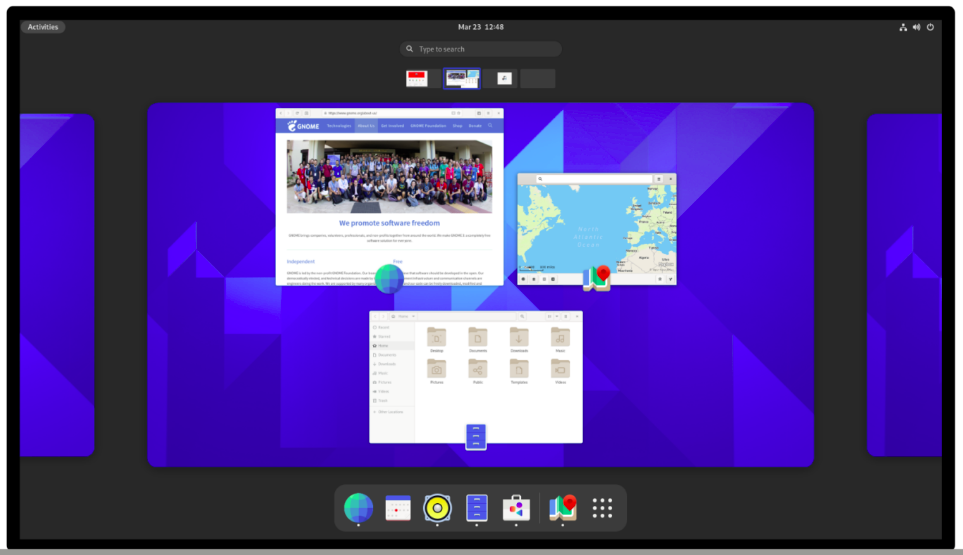
\includegraphics[width=250pt]{chapters/chapter1/figures/gnome_demo.png}
	\caption{GNOME desktop environment.} \label{ch1fig:gnomedemo}
\end{figure}

\begin{figure}
	\centering
	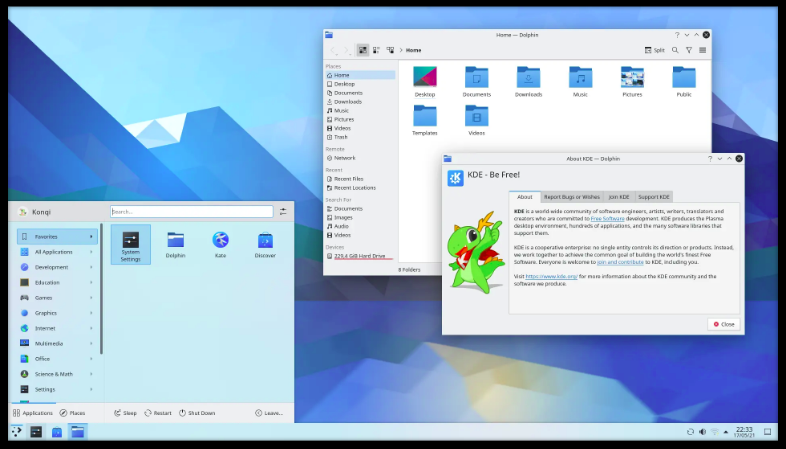
\includegraphics[width=250pt]{chapters/chapter1/figures/kde_demo.png}
	\caption{KDE desktop environment.} \label{ch1fig:kdedemo}
\end{figure}

\begin{figure}
	\centering
	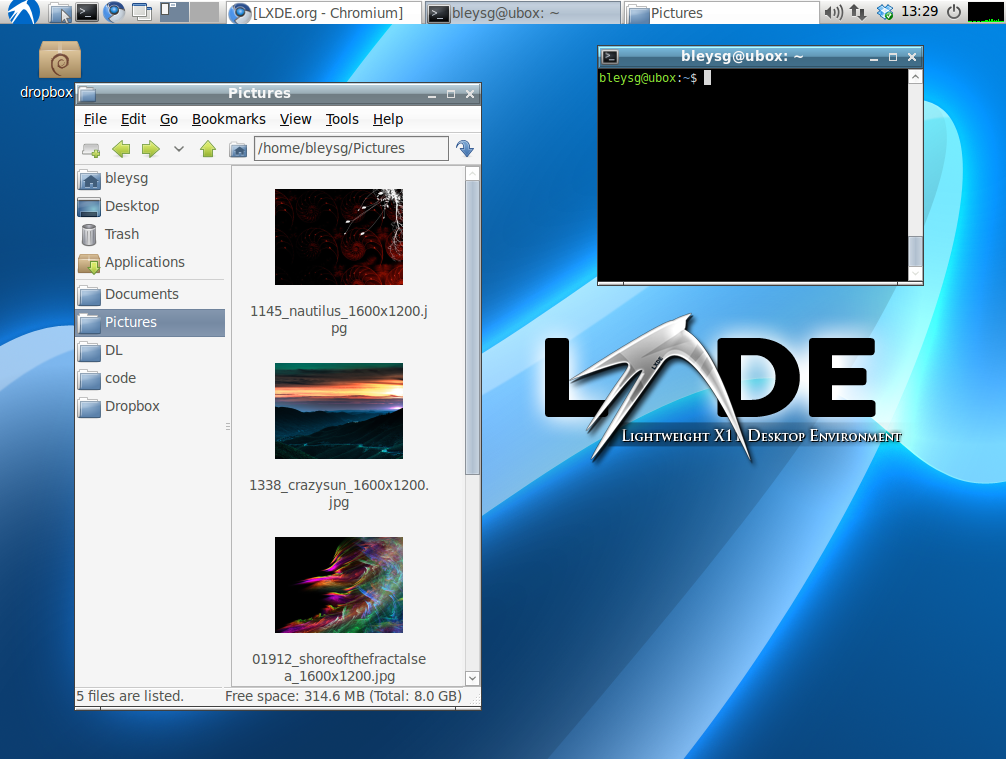
\includegraphics[width=250pt]{chapters/chapter1/figures/lxde_demo.png}
	\caption{LXDE desktop environment.} \label{ch1fig:lxdedemo}
\end{figure}

\begin{figure}
	\centering
	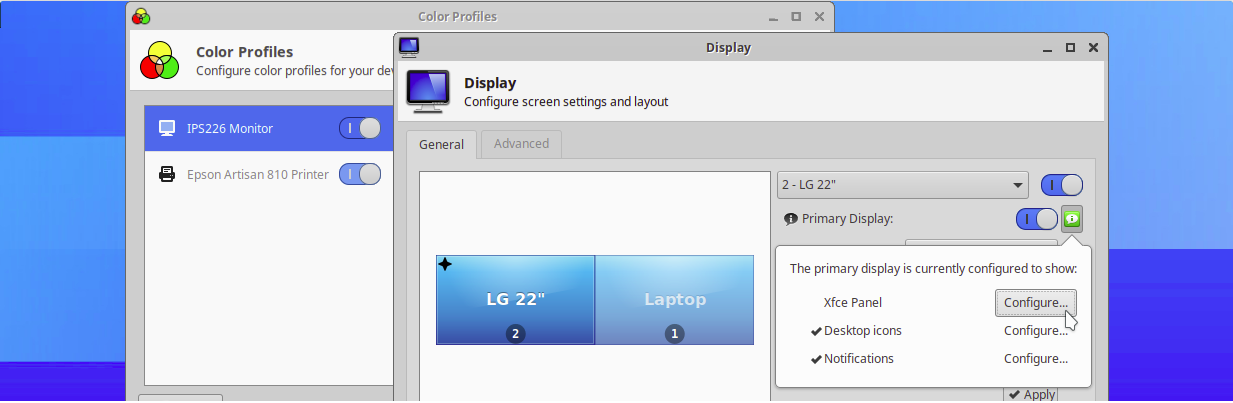
\includegraphics[width=250pt]{chapters/chapter1/figures/xfce_demo.png}
	\caption{Xfce desktop environment.} \label{ch1fig:xfcedemo}
\end{figure}

It is possible to install multiple desktop environment in one computer. In such a case, the user can choose which desktop environment to use each time the computer is powered on.

\section{Linux Installation}

Linux can be installed on a local PC hard disk, or on a mobile device such as a thumb drive. The installation of different distributions might differ. Thanks to the graphical installation tools for the popular distributions, the installations can be done easily by just following the instructions on the associated official sites.

Instructions of installing Ubuntu is given by \textit{https://ubuntu.com}

Instructions of installing Fedora is given by \textit{https://getfedora.org}

For the use of RHEL, consult with Red Hat at \textit{https://www.redhat.com}













% Shells Basics
%\chapterauthor{Author Name}{Author Affiliation}
%\chapterauthor{Second Author}{Second Author Affiliation}
\chapter{Shell}

Linux command line tool, usually known as the ``shell'', is the most powerful tool for Linux operations including configuration and control of the OS as well as other hardware/software of the system. Notice that the use of shell is not compulsory for casual users when the graphical desktop is present. Though the shell is not as intuitive as the graphical tools, the shell is more powerful and flexible, and well-supported by the community.

Linux shell will be used repeatedly in the remaining sections of this notebook for different functions.

\section{Brief Introduction}

Linux command line tool, usually known as Linux shell, was invented before the graphical tools, and it has been more powerful and flexible than the graphical tools from the first day. On those machines where no graphical desktops are installed, the use of shell is critical.

There are different types of shells. The most commonly used shell is the ``bash shell'' which stands for ``Bourne Again Shell'', derived from the ``Bourne Shell'' used in UNIX.

Some other shells such as ``C Shell'' and ``Korn Shell'' are also popular among certain users or certain Linux distributions. In case where your Linux distribution does not have these shells pre-installed, you can install and use these shells just like installing other software.

In this notebook, we will mostly focus on the bash shell.

\section{Basic Concepts}

After opening the shell or terminal, you will see a string (usually containing username, hostname, current working directory, etc.) followed by either a \verb|$| or \verb|#|, starting from where you can input your shell command. For example, it may look like the following:
\begin{verbatim}
username@hostname:~$
\end{verbatim}

The above displayed string is called a \textit{prompt}, indicating the start of a manually input command. By default, for regular user, the ending of the prompt is \verb|$| while for the root user, the ending is \verb|#|.

By saying root user, we are referring to a special user whose username and user ID (UID) ``root'' and $0$ respectively. This UID gives him the administration privilege over the machine, such as adding/removing users, change ownership of files etc. To avoid significant damage by human error, root user shall not be used unless it is definitely necessary. For this reason, in many servers the root user is deactivated (for example, by setting its login password to invalid).

Notice that a root user is different from regular user who is equipped with \textit{sudo privilege}, though a regular user with sudo privilege can temporarily switch to root user by using \verb|su| as follows.
\begin{verbatim}
regularuser@hostname:~$ sudo su
[sudo] password for regularuser:
root@hostname:/home/regularuser#
\end{verbatim}

More about sudo privilege, \verb|sudo| and \verb|su| commands are introduced later parts of the notebook.

You can key in a command after the prompt, and execute the command by pressing the \verb|Enter| key. A Linux shell command usually has the following form.
\begin{verbatim}
$ <command> <configuration-arguments> <input>
\end{verbatim}

\section{Useful Basic Commands}

Selected useful commands are categorized as follows. Notice that some commands have flexible use cases and it is impossible to illustrate all details about the commands. Consider use one of the following two methods to check the detailed manual about a command.
\begin{verbatim}
$ man <command>
$ <command> --help
\end{verbatim}

To execute a command, the command must have been stored somewhere in the PATH environment of the shell, which is usually initialized automatically when the shell is started. Check the PATH environment by
\begin{verbatim}
$ echo $PATH
<directory 1>:<directory 2>:<directory 3>: ...
\end{verbatim}
where \verb|echo| displays the content of a variable, and \verb|$PATH| is a build-in variable that records the PATH environment of the current bash. It is possible to include new directories to PATH environment either temporarily or permenently to enable new commands.

\vspace{0.1in}
\noindent \textbf{Show Login Information}
\vspace{0.1in}

Administrative users may need to frequently check the basic system information, such as hardware configuration, OS version, username, hostname, disk usage, running process, system clock, etc. Some useful commands are summarized below.

The following commands show basic information of a user.
\begin{verbatim}
$ whoami
<username>
$ grep <username> /etc/passwd
<username>:x:<uid>:<gid>:<gecos>:<home directory>:<shell> 
\end{verbatim}
In the above, \verb|whoami| is used to display the current login user's username. Consequently, \verb|grep| is used to search the user name in the selected file \verb|/etc/passwd| where the user information is stored. This should return the username, the password (for encrypted password, an ``x'' is returned), UID, group id (GID), user id info (GECOS), home directory and default shell location of the user.
Another command \verb|id| also returns the user id and group id information of the current user as follows.

The following commands show the date and hostname of the machine.
\begin{verbatim}
$ date
<date, time and timezone>
$ hostname
<hostname>
\end{verbatim}

\vspace{0.1in}
\noindent \textbf{Show Basic System Information}
\vspace{0.1in}

The following command \verb|lshw| lists down hardware information in details. Sudo privilege is recommended when using this command, to give detailed and accurate information of the system. Since the displayed information is so detailed and can take up many screens, sometimes it is more convenient to use \verb|-short| argument.
\begin{verbatim}
$ sudo lshw
\end{verbatim}



\vspace{0.1in}
\noindent \textbf{Navigate Files and Folders}
\vspace{0.1in}

The most important commands for navigating in the file system is to display the current working directory (may be included as part of prompt) and list down files and directories in the current working directory. The following commands do the work.
\begin{verbatim}
$ pwd
<absolute working directory>
$ ls
<a list of files/directories in the working directory>
\end{verbatim}

The aforementioned \verb|ls| command can be used flexibly. Commonly seen arguments that come with \verb|ls| are \verb|-l| (implement long listing with more details of each item), \verb|-a| (include hidden item in the list) and \verb|-t| (list by time).

\vspace{0.1in}
\noindent \textbf{Alias and Shortcuts}
\vspace{0.1in}

\section{Shell Environment Configuration}


\section{Shell Script Programming}















% Text file Editing
%\chapterauthor{Author Name}{Author Affiliation}
%\chapterauthor{Second Author}{Second Author Affiliation}
\chapter{Text File Editing}


\section{Text File Editing Environment in Linux}

\section{Vim}

\textit{Vim} is a free and open-source software initially developed by Bram Moolennar, and has become the default text editor of many Unix/Linux based operating systems.

Some people claim \textit{Vim} to be the most powerful text file editor as well as integrated development environment for programming on a Linux machine (and potentially on all computers and servers). The main reasons are as follows.
\begin{itemize}
  \item \textit{Vim} is usually built-in to Linux during the operating system installation, making it the most available and cost-effective text editor.
  \item \textit{Vim} can work on machines where graphical desktop is not supported.
  \item \textit{Vim} is light in size and is suitable to run even on an embedded system.
  \item \textit{Vim} operations are done mostly via mode switch and shortcut keys, so that \textbf{the brain does not need to halt and wait for the hand to grab and move the mouse} which slows down the text editing and interrupts the logic flow.
  \item \textit{Vim} is highly flexible and can be customized according to the user's habit (for example, through \verb|~/.vim/vimrc|), and it allows the users to define shortcut keys.
  \item \textit{Vim} can automate repetitive operations by defining macros.
  \item \textit{Vim} can be integrated with third-party tools for useful functions such as browsing project folders.
\end{itemize}
\textit{Vim} can be come very powerful and convenient for the user if he is very used to it. On the other hand, however, \textit{Vim} is not as intuitive as other text editors such as \textit{gedit} and \textit{notepad++}, and there might be a learning curve for beginners.

\subsection{General Introduction to Vim} \label{ch3:subsec:vimgeneralintro}

Unlike other text editors, \textit{Vim} defines different ``modes'' during the operation, each mode has some unique features. For example, in the \textit{insert} mode, \textit{Vim} puts keyboard inputs into the text file like an conventional text editor. In the \textit{normal} mode (this is the default mode when opening \textit{Vim}), \textit{Vim} uses useful and customizable shortcut keys to quickly navigate the document and perform operations such as cut, copy, paste, replace, search, and macro functions. In the \textit{virtual} mode, \textit{Vim} allows the user to select partial of the document for further editing. In the \textit{cmdline} mode, \textit{Vim} takes order from command lines and interact with Linux to perform tasks such as save, quit or even navigating folders.

The following Table \ref{ch3tab:vimmodes} summarizes the commonly used modes in Vim.
\begin{table}
  \centering \caption{Commonly used modes in \textit{Vim}.}\label{ch3tab:vimmodes}
  \begin{tabularx}{\textwidth}{lX}
    \hline
    Mode & Description \\ \hline
    Normal & Default mode. It is used to navigate the cursor in the text, search and replace text pieces, and run basic text operations such as undo, redo, cut (delete), copy and paste. \\ \hdashline
    Insert & It is used to insert keyboard inputs into the text, just like commonly used text editors today. \\ \hdashline
    Visual & It is similar to normal mode but areas of text can be highlighted. Normal mode commands can be used on the highlighted text. \\ \hdashline
    Cmdline & It takes in a single line command input and perform actions accordingly, such as save and quit. \\
    \hline
  \end{tabularx}
\end{table}

As a start, the following basic commands can be used to quickly create, edit and save a text file using vim. In home directory, start a shell and key in
\begin{verbatim}
$ vim testvim
\end{verbatim}
to create a file named ``testvim'' and open the file using \textit{Vim}. Notice that in some Linux versions, \textit{vi} might be aliased to \textit{vim} by default.

In the opened file, use \verb|Esc| and \verb|i|/\verb|a| to switch between normal mode and insert mode. In the normal mode, use \verb|h|, \verb|j|, \verb|k|, \verb|l| to navigate the position of the cursor. Finally, in the normal mode, use \verb|:w| to save the file, and \verb|:q| to quit \textit{vim}, or use \verb|:wq| to save and quit \textit{Vim}.

The above basic commands and their relationships are summarized in Fig.~\ref{ch3fig:vimbasicmodeswitching}. A flowchart to create/open, edit, save, and quit a text file using the aforementioned commands are given in Fig.~\ref{ch3fig:vimbasicoperationflowchart}.

\begin{figure}
\centering
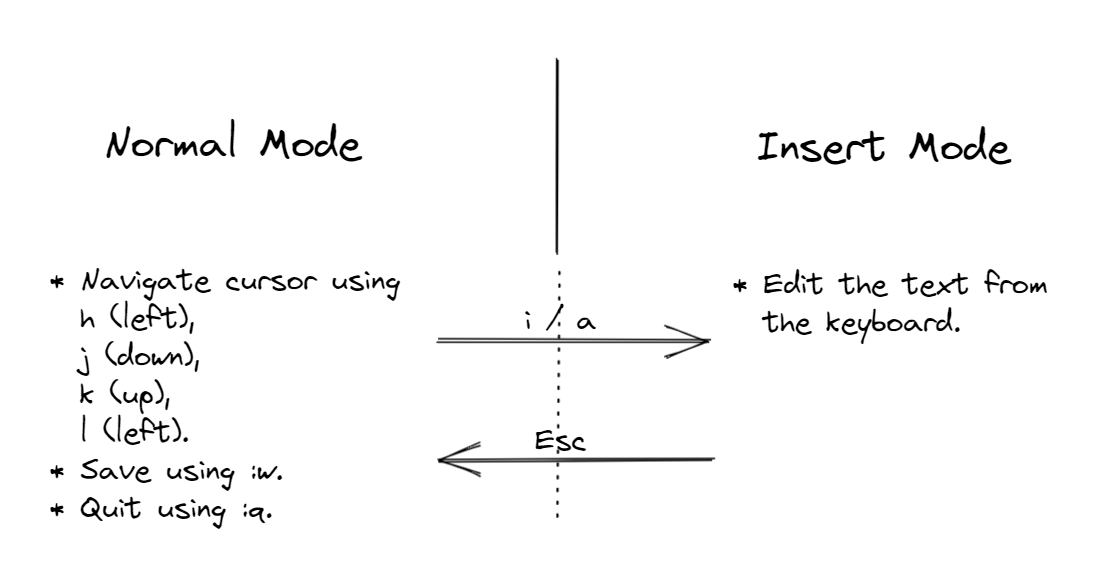
\includegraphics[width=250pt]{chapters/chapter3/figures/vimbasicmodeswitching.png}
\caption{Mode switching between normal mode and insert mode, and basic functions associated with the modes.} \label{ch3fig:vimbasicmodeswitching}
\end{figure}

\begin{figure}
\centering
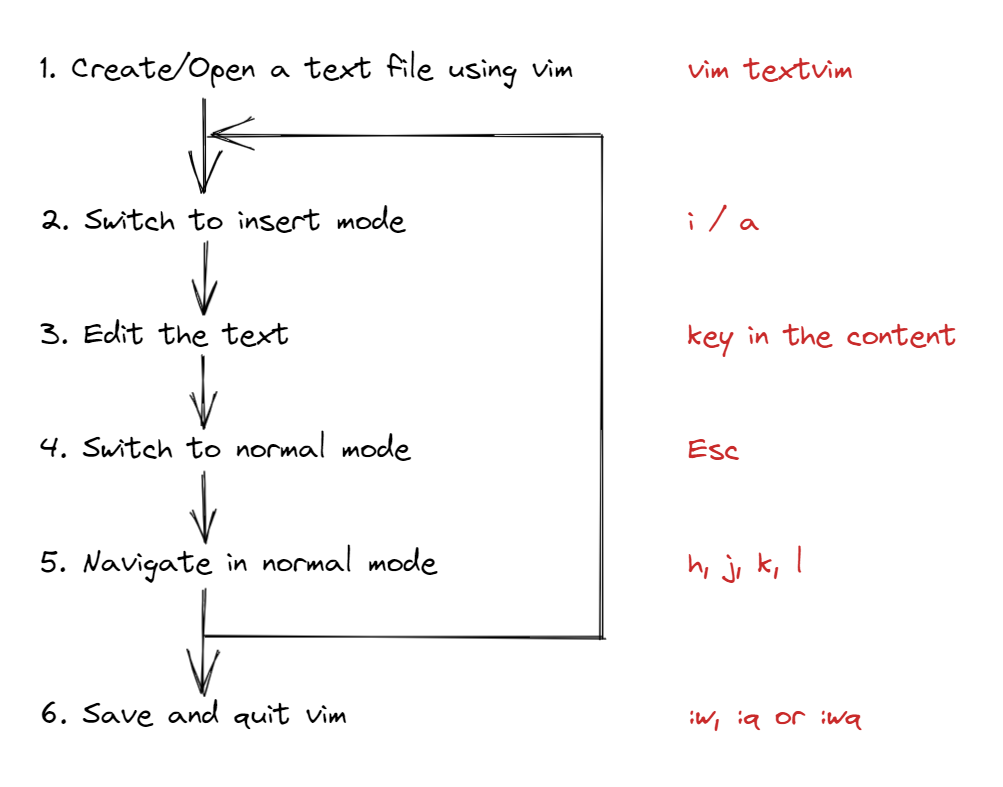
\includegraphics[width=250pt]{chapters/chapter3/figures/vimbasicoperationflowchart.png}
\caption{A flowchart for simple creating, editing and saving of a text file using \textit{Vim}.} \label{ch3fig:vimbasicoperationflowchart}
\end{figure}

There are other shortcuts to switch from normal mode to insert mode. Some of them are summarized in Table \ref{ch3tab:switchtoinsert}.

\begin{table}
  \centering \caption{Commonly used shortcuts to switch from normal mode to insert mode.}\label{ch3tab:switchtoinsert}
  \begin{tabularx}{\textwidth}{lX}
    \hline
    Operator & Description \\ \hline
    \verb|i| & Insert before the character at the cursor. \\ \hdashline
    \verb|I| & Insert at the beginning of the row at the cursor. \\ \hdashline
    \verb|a| & Insert after the character at the cursor. \\ \hdashline
    \verb|A| & Insert at the end of the row at the cursor. \\ \hdashline
    \verb|o| & Create a new row below the cursor and switch to insert mode. \\ \hdashline
    \verb|O| & Create a new row above the cursor and switch to insert mode. \\
    \hline
  \end{tabularx}
\end{table}

\subsection{Configure Customizable User Profile}

With the basic operations introduced in Section \ref{ch3:subsec:vimgeneralintro}, we are able to create and edit a text file as we want to, just like using any other text editor. Though at this point the advantages of using \textit{Vim} over other text editors are not obvious yet, the \textit{Vim} editor is at least useable.

Before introducing more advanced features of \textit{Vim} for more convenient user experience, we can now customize the user profile to suit our individual habit. Notice that the customization is completely optional and personal. This section only introduces the ideas and basic methods of such customization, such as re-mapping keys and create user-defined shortcuts. Everything introduced here are merely examples and it is completely up to the user how to design and implement his own profile.

In Linux, navigate to home directory. Create the following path and file \verb|~/.vim/vimrc| or \verb|~/.vimrc|. Open the \textit{vimrc} file as a blank file using \textit{Vim}. The individual user profile can be customized here.

\vspace{0.1in}
\noindent \textbf{Mapping of Keys}
\vspace{0.1in}

It is desirable to re-map some keys to speed up editing. For example, people may want to map \verb|jj| to \verb|Esc| in insert mode for more convenient mode switching to normal mode (consequent ``jj'' is rarely used in English). Other people may feel like mapping \verb|j|, \verb|k|, \verb|i| to \verb|h|, \verb|j|, \verb|k| respectively in normal and visual modes, making the navigation more intuitive. In that case, a different key needs to be mapped for \verb|i| since it is an important key for switching to insert mode.

It is possible re-map certain key (or keys combination) in selected modes. The following configuration in \textit{vimrc} file re-maps the aforementioned keys.
\begin{verbatim}
inoremap jj <Esc>
noremap j h
noremap J H
noremap k j
noremap K J
noremap i k
noremap I K
noremap h i
noremap H I
\end{verbatim}
where \verb|inoremap| is used to map keys (combinations) in insert mode, and \verb|noremap| in normal and visual modes.

The upper case letter \verb|S| and lower case letter |s| in control mode are originally used to delete and substitute texts. They may be not so important in practice as there functions are overlapped by another shortcut key \verb|c|, which is powerful in replacing characters and is more frequently used. We can re-map \verb|S| for saving the text, and disable \verb|s| to prevent mis-touching. Similarly, upper case letter \verb|Q| is mapped to quit \textit{Vim}.
\begin{verbatim}
noremap s <nop>
map S :w<CR>
map Q :q<CR>
\end{verbatim}
where \verb|<nop>| stands for ``no operation'' and \verb|CR| stands for the ``enter'' key on the keyboard. The keyword \verb|map| differs from \verb|noremap| in the sense that \verb|map| is for recursive mapping.

\vspace{0.1in}
\noindent \textbf{Syntax Highlight, Color Scheme and Others}
\vspace{0.1in}

By default \textit{Vim} displays white color contents on black background. Use the following command in \textit{vimrc} to enable syntax highlighting or change color scheme. Use \verb|:colorscheme| in normal mode in \textit{Vim} to check for available color schemes.
\begin{verbatim}
syntax on
colorscheme default
\end{verbatim}

The following command displays the row index and cursor line (a underline at cursor position) of the text, which can become handy during the programming. Furthermore, it sets auto-wrap of text when a single row is longer than the displaying screen.
\begin{verbatim}
set number
set cursorline
set wrap
\end{verbatim}

The following command opens a ``menu'' when using cmdline mode, making it easier to key in commands.
\begin{verbatim}
set wildmenu
\end{verbatim}

Many users in the community have posted their recommended \textit{Vim} user profile configuration online, such as on \textit{GitHub}. For the convenience of the reader, in the rest of the notebook, we will assume that \textbf{no re-map of keys combinations or shortcuts} are implemented, when introducing the commands.

Notice that the configurations introduced in this section can also be activated with the \textit{Vim} already started. Simply type \verb|:| to switch from normal mode to cmdline mode, then key in the configuration. For example, \verb|:syntax on| to activate the syntax display.

\subsection{Commonly Used Operations in Normal Mode}

The operations, such as delete, cut, copy, paste, replace and search, are mostly done in normal mode through shortcut keys. For example, \verb|dd| delete (cut) the entire row at the cursor and \verb|p| paste the row to its new position. For beginners, remembering shortcut keys can be difficult. In such case, it is recommended for us to look for the consistent patterns of the different commands, instead of brute-force remembering the keys only.

Many \textit{Vim} shortcut keys in normal mode has the following structure, i.e. an operator command followed by a motion command, as shown below.
\begin{verbatim}
<operator><motion>
\end{verbatim}
The operator command tells \textit{Vim} what to do (say, copy), and the motion command tells the applicable range of the operation (say, the entire row, or the single word, or the single character, of the cursor position). Of course for some operator commands, they can be used alone without the motion command.

\vspace{0.1in}
\noindent \textbf{Delete/Cut, Change, Copy and Paste}
\vspace{0.1in}

We will use the most commonly used operator commands, delete/cut, change, copy (also known as ``yank'' in \textit{Vim}) and paste to demonstrate the above idea.

In this demonstration, we will be editing the following lines taken from Wikipedia under ``William Shakespeare''. In the text file, each sentence takes a new row as given by Figure \ref{ch3fig:vimdemo1}.

\begin{shortbox}
William Shakespeare (bapt. 26 April 1564 – 23 April 1616) was an English playwright, poet and actor, widely regarded as the greatest writer in the English language and the world's greatest dramatist.

He is often called England's national poet and the ``Bard of Avon'' (or simply ``the Bard'').
\end{shortbox}

\begin{figure}
\centering
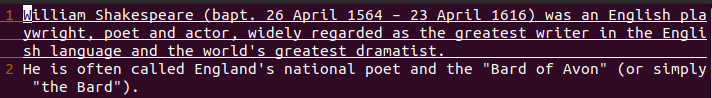
\includegraphics[width=250pt]{chapters/chapter3/figures/vimdemo1.png}
\caption{A piece of text of ``William Shakespeare'', for demonstration.} \label{ch3fig:vimdemo1}
\end{figure}

To quickly delete/cut a single character, use either \verb|x| or \verb|X|. Each time \verb|x| is input in normal mode, it deletes the current cursor selected character, and automatically select the next character in the text. Each time \verb|X| is input in normal mode, it keeps the current cursor selected character while deleting the previous character in front of the cursor. In this sense, \verb|x| and \verb|X| play like \verb|delete| and \verb|backspace| respectively in other text editors.

Operators \verb|x| and \verb|X| do not require consequent motion command, as they simply delete/cut one character immediately each time they are pressed. What if you want to delete multiple characters from the cursor? You can press \verb|x| or \verb|X| multiple times, or alternatively you can ask \textit{Vim} to do that repeatedly for you, as long as you tell \textit{Vim} what actions (key combinations) and how many times you want perform. For example, \verb|20x| is equivalent with physically pressing \verb|x| for 20 times. The same applies for other operators or motions commands. For example, \verb|10l| is equivalent of pressing \verb|l| for 10 times, making the navigation faster.

Operator \verb|d| does similar things as \verb|x| and \verb|X| but requiring a motion command, for more flexible usage. The motion shall tell \textit{Vim} what to delete/cut.

For example, \verb|dl| deletes to the right, i.e. deletes the current cursor selected character, and automatically select the next character. It is the same as if \verb|x| is pressed. Similarly, \verb|dh| deletes  to the left, just like \verb|X|. What if you want to delete 20 characters to the right? You can key in \verb|dl| for 20 times. Or alternatively, just like the case for \verb|x|, you can tell \textit{Vim} to do it by using \verb|20dl|. Or, you can change the motion, by using \verb|d20l|, where ``20l'' as a whole plays as the motion of ``to the right for 20 characters''. Or, you can do a combination by using things like \verb|5d4l|, since $20=5\times 4$. All of the above gives you the same result (they will be a difference in the clipboard if later you want to paste them).

Thanks to the ``operator-motion'' structure, \verb|d| can be used even more flexibly. For example, by using word-related motions, \verb|d| can delete/cut by words instead of by characters. Move the cursor to the beginning of a word, (for example, ``S'' in ``Shakespeare''), use \verb|dw| to delete the word. The word motion \verb|w| is similar with \verb|l|, except that \verb|l| directs to the next character, while \verb|w| directs to the beginning character of next word. Motion \verb|w| can also be used to navigate in the text. Similarly, \verb|b| directs to the beginning character of the current word (if the cursor is at the middle of the current word) or previous word (if the cursor is already at the beginning of the current word). Thus, \verb|db| can be used to delete word to the left. You can use something like \verb|d10b|, \verb|10db|, \verb|d20w|, \verb|5d4w| to delete multiple words at a time.

When in the middle of a word, \verb|dw| will delete the characters from the current cursor position till the beginning character of the next word. For example, if the cursor is currently at ``k'' in ``Shakespeare'', \verb|dw| will delete ``kespeare '' (notice that the space between ``Shakespeare'' and ``(bapt.'' will also be deleted). To delete from the beginning of the word instead of from the middle of the word, you can use \verb|b| first to navigate back to the beginning of the word. Alternatively, use ``inner-word'' motion \verb|iw| to indicate that you want to delete inner word. When the cursor is at ``k'' in ``Shakespeare'', use \verb|diw| to delete the entire word.

So far we have introduced the delete/cut operator \verb|d|, and character motion \verb|h| (left), \verb|l| (right), and also word motion \verb|b| (left), \verb|w| (right). There are similar motions for sentence \verb|(| (previous), \verb|)| (next) and paragraph \verb|{| (previous), \verb|}| (next). Finally, there is the inner-word motion \verb|iw| to indicate the current word of cursor, whichever the cursor is inside the word. Similarly, there are inner-sentence motion \verb|is| and inner-paragraph motion \verb|ip|. There are also inner-quotation motion \verb|i'|, \verb|i"|, \verb|i`| and inner-block motion \verb|i(|, \verb|i<|, \verb|i{|, and many more. For example, when cursor is at ``A'' of ``26 April 1564'', \verb|di(| will delete everything inside ``()'', i.e. deleting ``bapt. 26 April 1564 - 23 April 1616''.

To conclude, the operators and motions so far are listed in Tabs. \ref{ch3tab:deletecut} and \ref{ch3tab:motion}. Notice that motions \verb|aw|, \verb|as|, \verb|ap| are also given in the table. They are similar with their corresponding \verb|iw|, \verb|is|, \verb|ip| except that when deleting, the consequent blank space (for word and sentence) or blank row (for paragraph) will also be deleted. (Notice that \textit{Vim} marks the end of a sentence using ``.'', ``?'' or ``!'' followed by a space, tab or blank row, and the end of a paragraph by an empty row.)

\begin{table}
  \centering \caption{Commonly used operators related to delete/cut, change, copy and paste.}\label{ch3tab:deletecut}
  \begin{tabularx}{\textwidth}{lX}
    \hline
    Operator & Description \\ \hline
    \verb|x| & Delete/Cut the character at cursor. \\ \hdashline
    \verb|X| & Delete/Cut the character before cursor. \\ \hdashline
    \verb|dd| & Delete/Cut the entire row. \\ \hdashline
    \verb|d| & Delete/Cut selected text according to the motion command. \\ \hdashline
    \verb|cc| & Change the entire row. \\ \hdashline
    \verb|c| & Change selected text according to the motion command. \\ \hdashline
    \verb|yy| & Copy the entire row. \\ \hdashline
    \verb|y| & Copy selected text according to the motion command. \\ \hdashline
    \verb|p| & Paste clipboard to the cursor. \\
    \hline
  \end{tabularx}
\end{table}

\begin{table}
  \centering \caption{Commonly used motions.}\label{ch3tab:motion}
  \begin{tabularx}{\textwidth}{lX}
    \hline
    Motion & Description \\ \hline
    \verb|h|, \verb|l| & One character to the left or right. \\ \hdashline
    \verb|j|, \verb|k| & One row to the up or down. \\ \hdashline
    \verb|b|, \verb|w| & One word to the previous or next. \\ \hdashline
    \verb|(|, \verb|)| & One sentence to the previous or next. \\ \hdashline
    \lstinline{\{}, \lstinline{\}} & One paragraph to the previous or next. \\ \hdashline
    \verb|iw|, \verb|is|, \verb|ip| & inner-word, inner-sentence, inner-paragraph. \\ \hdashline
    \verb|aw|, \verb|as|, \verb|ap| & a word, a sentence, a paragraph (including the end blank). \\ \hdashline
    \verb|i'|, \verb|i"|, \verb|i`| & inner-quotation for different types of quotations. \\ \hdashline
    \verb|i(|, \verb|i<|, \verb|i[|, \lstinline{\}} & inner-block for different types of brackets. \\ \hdashline
    \verb|0| & Beginning of the row. \\ \hdashline
    \verb|$| & Ending of the row. \\ \hdashline
    \verb|gg| & Beginning of the text. \\ \hdashline
    \verb|G| & Beginning of the last row of the text. \\
    \hline
  \end{tabularx}
\end{table}

To change a piece of text, operator \verb|c| is used, followed by its associated motion to indicate the range of text to be changed. The same motions as given in Table \ref{ch3tab:motion} can be used. Effectively, operator $\verb|c|$ deletes/cut the text indicated by the motion first (just like operator \verb|d|), then switch to insert mode.

To copy a piece of text of clipboard, use \verb|y| (stands for ``yank'') followed by its associated motion to indicate the range of text. The motions also follow Table \ref{ch3tab:motion}.

To paste the text in the clipboard to the text at the cursor position, use \verb|p|. No motion is required.

In addition to the motions given in Table \ref{ch3tab:motion}, another commonly used method to navigate to a particular position if text is to ``find by character''. For example, consider the following row of text. The cursor is currently at letter ``A''.
\begin{verbatim}
ABCDEFG;HIJKLMN;OPQ;RST;UVW;XYZ
\end{verbatim}
In normal mode, using \verb|f| followed by a character will navigate the cursor to the nearest corresponding character that appears in the text. For example, \verb|fG| will move the cursor to letter ``G''. Similarly, \verb|f;| will move the cursor to the ``;'' between ``G'' and ``H''. Key in \verb|f;| again and the cursor will move to ``;'' between ``N'' and ``O''. From here key in \verb|2f:| and the cursor will go to ``;'' between ``T'' and ``U'', as it is equivalent to typing \verb|f;| twice.

\vspace{0.1in}
\noindent \textbf{Search in the Text}
\vspace{0.1in}

It is common that we want to search for a particular keywords or phrase, and highlight all of its appearances in the text. To make the searching result highlighted, add the following line to the user profile at \textit{vimrc}.
\begin{verbatim}
set hlsearch
exec "nohlsearch"
set incsearch
set ignorecase
\end{verbatim}
where \verb|hlsearch| highlights all matching results in the text, and \verb|incsearch| allows highlighting texts while keying in the word or phrase. Each time highlight search is enabled, \textit{Vim} will remember the keywords from the previous search and automatically hight them in the text, which can be confusing sometimes. The command \verb|exec "nohlsearch"| (\verb|exec| command in the user profile make \textit{Vim} execute that command when starting a new session) that comes after \verb|set hlsearch| resolves this issue by forcing \textit{Vim} to clear its memory. Finally, \verb|ignorecase| allows case insensitive while searching.

In normal mode, use \verb|/<keyword>| to search keywords or phrase. With the above setup, search for ``he'' using \verb|/he| will lead to the following result given in Fig.~\ref{ch3fig:vimdemo2}.
\begin{figure}
\centering
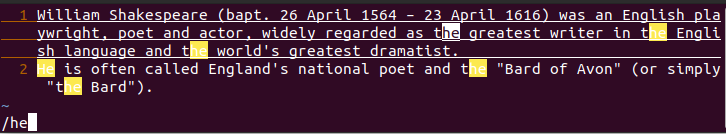
\includegraphics[width=250pt]{chapters/chapter3/figures/vimdemo2.png}
\caption{Search ``he'' in the piece of text of ``William Shakespeare''.} \label{ch3fig:vimdemo2}
\end{figure}
From Fig.~\ref{ch3fig:vimdemo2}, it can be seen that all appearances of ``he'' (case insensitive) is highlighted, and the cursor is automatically moved to the first appearance, i.e. ``he'' in ``and the world's greatest dramatist''. Click \verb|Enter| to quit searching. Now \verb|h|, \verb|j|, \verb|k| and \verb|l| can be used to navigate the cursor again, with the searching result maintain highlighted. Use \verb|n| and \verb|N| to navigate the cursor from the highlighted results. Notice that in this case, \verb|n| and \verb|N| can be used as motion together with delete/cut, change and copy as given in Table \ref{ch3tab:deletecut}.

To disable the existing searching highlight, either start searching a new keyword, or key in command \verb|:nohlsearch| in normal mode. For convenience, people may prefer to map it with a customized shortcut key as well, for example in \textit{vimrc} key in
\begin{verbatim}
noremap <Space> :nohlsearch<CR>
\end{verbatim}
so that \verb|Space| can be used to clear the search highlights.

\vspace{0.1in}
\noindent \textbf{Visual Mode}
\vspace{0.1in}

The use of a mouse makes selecting a block of text very intuitive. As your eyes move across the text, you can start selecting at any specific character or row by click-and-hold the mouse key, and end selecting at any specific character or row by simply letting it go. The selected text will be highlighted, as if the cursor expands from one character to the entire block of text. You can then perform operations such as delete or copy of the selected block of text.

When using \textit{Vim}, mouse is mostly useless. The visual mode of \textit{Vim} provides users a similar experience when selecting a block of text almost as if using a mouse.

It is possible to select multiple rows of text in visual mode, and then apply an operation all at rows simultaneously.



\subsection{Advanced Interface}


\subsection{Vim Accessories}





% Managing files
\chapter{Applications}

This chapter introduces some interesting and widely known use cases of derivatives and integrals. 

Section \ref{ch4sec:newtonsmethod} introduces Newton's method, a widely used numerical method to solve equation $f(x) = 0$ for some continuous function $f(x)$. 

Section \ref{ch4sec:taylorseries} introduces Taylor serious, a widely used numerical method to approximate the value of $f(x)$ near a specific $x_0$.

\section{Newton's Method} \label{ch4sec:newtonsmethod}

Consider solving an equation $f(x)=0$ for continuous function $f(x)$. Sometimes it is possible to construct a function $g(x)$, such that $x= x + g(x)$ has the same solution with $f(x) = 0$. Equation $f(x)=0$ might then be solved recursively using $x^{k+1} = x^k + g(x^k)$ where $k$ is the recursive index. In this notebook, we are not going to discuss how $g(x)$ can be constructed and what limitations of this method may have.

In Newton's method, $g(x)$ is constructed as $g(x) = -\frac{f(x)}{f^\prime(x)}$. For Newton's method to converge to the correct solution, there is some restrictions to $f(x)$ and also the choice of $x^0$ as the initial guess. The detailed discussion to these restrictions are not covered in this notebook.

The basic procedures for Newton's method are given below.

\textbf{Step 1: Determine a feasible range $[a, b]$ where the solution to $f(x)=0$ must lie inside.} This can be done by having a rough guess of an range $[a, b]$ near the solution, and make sure $f(a)f(b)<0$. It can be proved that for a continuous function $f(x)$, $f(a)f(b)<0$ guarantees a solution in $[a, b]$.

\textbf{Step 2: Have a initial guess $x^0 \in [a, b]$. Initialize $k=0$.}

\textbf{Step 3: Calculate $f^\prime(x^k)$, then calculate $x^{k+1}$ as follows.}
\begin{eqnarray}
    x^{k+1} &=& x^k - \dfrac{f(x^k)}{f^\prime(x^k)}. \nonumber
\end{eqnarray}

Step 3 is iterated to for recursive calculation of $x^{k}$. The iterations stops when either of the following happens: (a) $|f(x^k)| < \varepsilon$; or (b) $|x^{k+1}-x^k|<\varepsilon$, where $\varepsilon$ is a pre-defined threshold parameter. The finally calculated $x^k$ is the numerical solution of the original equation $f(x)=0$ using Newton's method.

\section{Taylor Series} \label{ch4sec:taylorseries}

Consider a continuous and $(n+1)$-th order differentiable function $f(x)$ defined on interval $[a, b]$. Taylor series introduces a way to approach a function $f(x)$ at any $x \in [a, b]$ using a sum of sequence consisting $f(x)$ and its derivatives at a particular $x_0 \in [a, b]$.

Taylor series claims that such $f(x)$ can be expressed by the following equation
\begin{eqnarray}
    f(x) &=& P(x,x_0), + R(x,x_0), \label{ch4eq:taylorseries}
\end{eqnarray}
where
\begin{eqnarray}
    P(x,x_0) &=& \sum_{k=0}^n \dfrac{f^{(k)}(x_0)}{k!}(x-x_0)^k, \nonumber \\
    R(x,x_0) &=& \dfrac{f^{(n+1)}\left(x_0 + \theta(x-x_0)\right)}{(n+1)!}(x-x_0)^{n+1}, \label{ch4eq:taylorseriesremainder}
\end{eqnarray}
with $\theta \in (0,1)$, and $f^{(n)}(x)$ the $n$-th order derivative of $f(x)$, i.e. ``the derivative of derivative of ... derivative of $f(x)$'', where there are $n$ ``derivative'' in the sentence.

Equation \eqref{ch4eq:taylorseries} uses $P(x,x_0)$ to approximate $f(x)$. It can be seen from \eqref{ch4eq:taylorseriesremainder} that with $n\rightarrow \infty$ or $x \rightarrow x_0$, the remainder $R(x,x_0) = f(x) - P(x,x_0)$ approaches zero (notice that $f^{(n+1)}$ is assumed bounded). This implies that the approximation performs better when higher order Taylor series is used, or when the target point $x$ is close to the evaluated point $x_0$.

The following Fig. \ref{ch4fig:taylordemo} gives an example of using Taylor series to approximate function $y=2^x$ at $x_0=0$. In this example, it can be seen that the approximation gets better when higher order Taylor series is used.
\begin{figure}
\centering
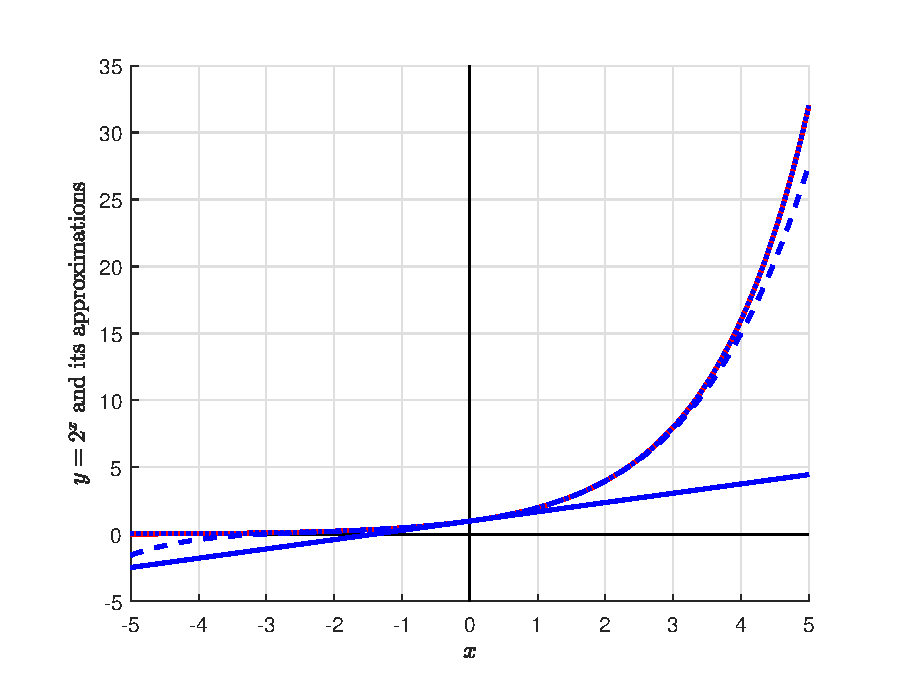
\includegraphics[width=250pt]{chapters/chapter4/figures/taylorseriesexp.eps}
\caption{Plot of function $y=2^x$ in red solid line, and its approximations using first-order, $5$th-order and $10$th-order Taylor series in blue solid line, blue dashed line and blue dot line respectively.} \label{ch4fig:taylordemo}
\end{figure}

For polynomial functions $f(x)$, $f^{(n)}(x) = 0$ for large enough $n$, depending on the degree of the polynomial. For a $N$-th-order polynomial, $f^{(n)}(x) = 0$ for $n>N$, thus its $n$-th-order (or higher) Taylor series $P(x,x_0)=f(x)$ for any choice of $x_0$.


% Managing Software
\chapter{Multivariable Function}

This chapter introduces functions with multiple inputs and/or outputs. Usually, these inputs and outputs are put into vectors for computation and presentation convenience. Section \ref{ch5sec:briefintrotovectormatrix} gives a very brief introduction to the basics of vector and matrix operations. Section \ref{ch5sec:multivarfunction} introduces the concept of multivariable functions, including the multiple input function and the vector function.

From calculus perspective, this chapter clears the preliminary knowledge required for later Chapters \ref{ch6ch} and \ref{ch7ch}.

\section{Brief Introduction to Vector and Matrix} \label{ch5sec:briefintrotovectormatrix}

Detailed introduction to vector and matrix can be found in any \textit{linear algebra} textbook, where there are the geometric interpretation of vector, then linear equation represented by product of matrix and vector, then column and null space of matrix, then rank of matrix and determinant of square matrix, then inverse of matrix, then linear transformation of matrix, then eigenvalue of matrix, then norm of vector and matrix, then algebraic Riccati equation, and so on. This list can go almost eternally. To make things even more complicated, depending on the application, the vector and matrix may have different physical meanings. For example, the speed of motion and the bus voltage phasors of a microgrid can all be represented by vectors, but might be completely two different things.

In the context of this notebook, however, most of the above are out of the scope. We will take vector and matrix as a way of organizing scalar data. Basically, a vector is a 1-D chain of scalar variables, and a matrix is a 2-D rectangular mesh of scalar variables. In many cases such as calculating matrix product, a vector can be taken as a special case of matrix, and a scalar is a special case of a vector. Of course, the very basics such as product of matrices are still required.

The preliminary vector and matrix knowledge used in this notebook is summarized in the rest of this section as follows.

\subsection{Basic Concepts}

A vector $x$ (sometimes denoted as bold text $\textbf{x}$ in textbooks) is a finite sequence of scalar variables organized in a 1-D chain. The length of the vector, or the dimension of the vector, is the number of elements in the vector. For vector $x$ with $n$ elements, the elements are denoted by $x_1, x_2, \cdots, x_n$, and $x_i$ is called the $i$-th element of the vector.

Most of the vectors in this notebook are by default \textit{column vectors}, which means that the $n$ elements are put into $n$-row-$1$-column, as follows. In this case, we say \textit{``$x$ is a $n$ dimensional column vector''} or \textit{``$x$ is a $n\times 1$ vector''}.
\begin{eqnarray}
    x &=& \left[\begin{array}{cc}
         x_1  \\
         x_2 \\
         \vdots \\
         x_n
    \end{array}\right]. \label{ch5eq:columnvector}
\end{eqnarray}

A row vector, on the other hand, puts the $n$ elements into $1$-row-$n$ column. A row vector is like a column vector flipped diagonally, as shown below in \eqref{ch5eq:rowvector}. We call the flipping operation \textit{``transpose''}, denoted by $(\cdot)^T$ (used in this textbook) or $(\cdot)^\prime$.
\begin{eqnarray}
    x^T &=& \left[\begin{array}{cccc} x_1 & x_2 & \ldots & x_n
    \end{array}\right], \label{ch5eq:rowvector}
\end{eqnarray}
where $x^T$ is a row vector and it is a transpose of the column vector $x$ previously given in \eqref{ch5eq:columnvector}. The transpose of a column vector is a row vector, and vise versa. The transpose of a scalar is itself.

A matrix $A$ (sometimes denoted as bold $\textbf{A}$ in textbooks) is a finite number of scalar variables organized in 2-D mesh, with each scalar taking a particular position. The number of rows and columns are the dimension of the matrix. For example, if $A$ has $m$ rows and $n$ columns, we say \textit{``$A$ has a dimension of $m\times n$''} or \textit{``$A$ is a $m\times n$ matrix''}, shown as follows.
\begin{eqnarray}
    A &=& \left[\begin{array}{cccc}
        a_{1,1} & a_{1,2} & \ldots & a_{1,n} \\
        a_{2,1} & a_{2,2} & \ldots & a_{2,n} \\
        \vdots & \vdots & \ddots & \vdots \\
        a_{m,1} & a_{m,2} & \ldots & a_{m,n}
    \end{array}\right], \label{ch5eq:matrixa}
\end{eqnarray}
where $a_{i,j}$ is the $i$-th row, $j$-th column element of $A$.

The transpose operation is also defined on matrix. By applying transpose on $A$ in \eqref{ch5eq:matrixa}, a $n\times m$ matrix $A^T$ can be obtained, where the $i$-th row, $j$-th column element in the transpose matrix $A^T$ is the $j$-th row, $i$-th column element in the original matrix $A$.

The vectors or matrices with the same dimension can be added together by adding each associated pair of elements together.

\subsection{Matrix Multiplication}

The product of two matrices is defined as follows. 

\begin{VF}
\textbf{Matrix Multiplication}:
\\
\\
Consider matrices $A$ and $B$. As a prerequisite of calculating $AB$, the number of column in the first matrix $A$ must equal to the number of row in the second matrix $B$. 

Let $A$ and $B$ be $m\times p$ matrix and $p\times n$ matrix respectively. The matrix product $C=AB$ is a $m \times n$ matrix with each element calculated by

\begin{eqnarray}
    c_{i,j} &=& a_{i,1}b_{1,j} + a_{i,2}b_{2,j} + \ldots + a_{i,p}b_{p,j} \nonumber \\
    &=& \sum_{k=1}^p a_{i,k}b_{k,j}, \nonumber
\end{eqnarray}
for $i = 1, \ldots, m$ and $j= 1, \ldots, n$.

It is clearly from the definition that $AB$ does not equal to $BA$. In the example above, if $m\neq n$, $BA$ does not exist in the first place.
\end{VF}

It can be proved by definition that if $C=AB$, $C^T = (AB)^T = B^TA^T$.

In terms of matrix multiplication, a vector is just a special case of matrix. Therefore, the product of a matrix with a vector $y=Ax$ where $A$ is a $m\times n$ matrix and $x$ a $n\times 1$ matrix, is a $m\times 1$ vector given by
\begin{eqnarray}
    y &=& Ax \nonumber \\
    &=& \left[\begin{array}{cccc}
        a_{1,1} & a_{1,2} & \ldots & a_{1,n} \\
        a_{2,1} & a_{2,2} & \ldots & a_{2,n} \\
        \vdots & \vdots & \ddots & \vdots \\
        a_{m,1} & a_{m,2} & \ldots & a_{m,n}
    \end{array}\right] \left[\begin{array}{cc}
         x_1  \\
         x_2 \\
         \vdots \\
         x_n
    \end{array}\right] \nonumber \\
    &=& \left[\begin{array}{c}
         \sum_{k=1}^n a_{1,k}x_k \\
         \sum_{k=1}^n a_{2,k}x_k \\
         \vdots \\
         \sum_{k=1}^n a_{m,k}x_k
    \end{array}\right]. \nonumber
\end{eqnarray}

The product of row vector $u^T$ and column $v$, both $n$ dimensional vectors, is
\begin{eqnarray}
    u^Tv &=& \left[\begin{array}{cccc} u_1 & u_2 & \ldots & u_n
    \end{array}\right] \left[\begin{array}{cc}
         v_1  \\
         v_2 \\
         \vdots \\
         v_n
    \end{array}\right] \nonumber \\
    &=& \sum_{k=1}^n u_kv_k \nonumber
\end{eqnarray}
which is a scalar. As a special case, $x^Tx = \sum_{k=1}^n x_i^2$ for a $n$ dimensional vector $x$.

\subsection{Block Matrix}

For the convenience of calculation and interpretation, sometimes a large dimension matrix is split into a combination of smaller dimension sub matrices.

For example, consider matrix $A$ with dimension $m \times p$ and matrix $B$ with dimension $p\times n$. Matrix $A$ can be split into two sub matrix $A_1$ and $A_2$, where $A_1$ consists of the first $m_1$ rows of $A$ thus $m_1 \times p$ dimension, and $A_2$ consists of the rest $m_2 = m - m_1$ rows of $A$ thus $m_2\times p$ dimension, i.e.
\begin{eqnarray}
    A &=& \left[\begin{array}{c}
         A_1  \\
         A_2 
    \end{array}\right]. \nonumber
\end{eqnarray}
The calculation of $C=AB$ can be done as follows
\begin{eqnarray}
    C = AB = \left[\begin{array}{c}
         A_1  \\
         A_2 
    \end{array}\right]B = \left[\begin{array}{c}
         A_1B  \\
         A_2B 
    \end{array}\right]. \nonumber
\end{eqnarray}

Similarly, if split matrix $B$ into two sub matrices, with $B_1$ the first $n_1$ columns and $B_2$ the rest $n_2 = n - n_1$ columns of $B$, then
\begin{eqnarray}
    C = AB = A \left[\begin{array}{cc}
        B_1 & B_2 
    \end{array}\right] = \left[\begin{array}{cc}
        AB_1 & AB_2 
    \end{array}\right] \nonumber
\end{eqnarray}

Furthermore, splitting both $A$ and $B$ simultaneously gives
\begin{eqnarray}
    C = AB = \left[\begin{array}{c}
         A_1  \\
         A_2 
    \end{array}\right] \left[\begin{array}{cc}
        B_1 & B_2 
    \end{array}\right] = \left[\begin{array}{cc}
        A_1B_1 & A_1B_2 \\
        A_2B_1 & A_2B_2
    \end{array}\right] \label{ch5eq:blockmatrixproduct}
\end{eqnarray}
Equation \eqref{ch5eq:blockmatrixproduct} sometimes helps to speed up the matrix product as it allows to split the calculation into independent pieces. But more importantly, equation \eqref{ch5eq:blockmatrixproduct} gives a lot of insights into matrix operations and linear transformation. The details are not covered in this notebook.

\subsection{Identity Matrix and Square Matrix Inverse}

A matrix is called a \textit{square matrix} if it has the same number of rows and columns. For example, if matrix $A$ has a dimension of $n\times n$, then it is a square matrix of dimensional $n$. The elements with the same row and column index, i.e. $a_{i,i}, i=1, \ldots, n$, are called the diagonal elements.

The \textit{identity matrix}, denoted by $I$, is a special type of square matrix as given in \eqref{ch5eq:identitymatrix}. Its diagonal elements are $1$, with the rest elements $0$. 
\begin{eqnarray}
    I &=& \left[\begin{array}{ccccc}
        1 & 0 & 0 & \ldots & 0 \\
        0 & 1 & 0 & \ldots & 0 \\
        0 & 0 & 1 & \ldots & 0 \\
        \vdots & \vdots & \vdots & \ddots & \vdots \\
        0 & 0 & 0 & \ldots & 1
    \end{array}\right] \label{ch5eq:identitymatrix}
\end{eqnarray}

A $n$ dimensional identity matrix is denoted by $I_n$. The multiplication of the identity matrix with any matrix from either left or right side does not change the matrix, i.e. for any matrix $A$ with dimension $m\times n$, $I_{m}A = AI_{n}=A$.

A square matrix may have an associated inverse matrix. The definition of inverse matrix is given as follows.

\begin{VF}
\textbf{Definition of inverse of a matrix}:
\\
\\
Consider a square matrix $A$ with dimension $n\times n$. Matrix $A$ is called \textit{invertible} if such matrix $A^{-1}$ with dimension $n\times n$ exists that
\begin{eqnarray}
    AA^{-1} = A^{-1}A = I_n, \nonumber
\end{eqnarray}
and $A^{-1}$ is called the \textit{inverse} of matrix $A$.

\end{VF}

Notice that matrix $A^{-1}$ may not exist for some $A$, depending on the determinant of $A$. Details can be found in linear algebra textbooks and are not given in this notebook.

\section{Multivariable Function} \label{ch5sec:multivarfunction}

In Chapters 2 and 3, we have been considering single-input-single-output functions only, i.e. for function $y=f(x)$, we have been discussing only the cases where $y$ and $x$ are scalars so far.

In many other cases, however, a function may have multiple input and/or output variables. For example, consider the following function used to calculate the mechanical energy of an object
\begin{eqnarray}
    e = f(v, h) = \dfrac{1}{2}mv^2 + mgh. \nonumber
\end{eqnarray}
where $m$, $v$ and $h$ are the mass, motion speed and height (related to ground) of the object, and $g$ is the free-fall acceleration, $g=9.8m/s^2$ on the earth. This is a typical multivariable function, where the function $z=f(x, y)$ depends on multiple independent variables $x$ and $y$.

When there are multiple outputs for a function, the outputs are often out into a column vector and the function is called a \textit{vector function}. Two examples of vector functions are given below.
\begin{eqnarray}
    f(x) &=& \left[\begin{array}{cc}
        1 & 0 \\
        0 & 1 \\
        3 & -2
    \end{array}\right]x, \label{ch5eq:vectorlinear} \\
    g(x) &=& \left[\begin{array}{c}
         g_1(x)  \\
         g_2(x)
    \end{array}\right] = \left[\begin{array}{c}
         x_1^2 + x_2^2  \\
         0.5x_1 + e^{x_2}
    \end{array}\right], \label{ch5eq:vectornonlinear}
\end{eqnarray}
where $f(x)$ and $g(x)$ are both vectors with dimension $3\times 1$ and $2\times 1$ respectively. Equation \eqref{ch5eq:vectorlinear} is a linear function with $2$ inputs $x = \left[\begin{array}{cc}
    x_1 & x_2
\end{array}\right]^T$ and $3$ outputs $y = \left[\begin{array}{ccc}
    y_1 & y_2 & y_3
\end{array}\right]^T$, while \eqref{ch5eq:vectornonlinear} is a nonlinear function with $2$ inputs $x = \left[\begin{array}{cc}
    x_1 & x_2
\end{array}\right]^T$ and $2$ outputs $g = \left[\begin{array}{cc}
    g_1 & g_2
\end{array}\right]^T$.





% Managing Task
\chapter{Partial derivative} \label{ch6ch}

Partial derivative studies the effect of a small deviation of one particular independent variable on the multivariable function. It is similar with the normal derivative in many ways, but also has its unique characteristics.

In Section \ref{ch6sec:motivatingexp}, a motivating example is given to illustrate the motivation of introducing partial derivative. In Section \ref{ch6sec:partialtotalderivative}, the definition of partial derivative is given. In Sections \ref{ch6sec:gradient} and \ref{ch6sec:jacobianmatrix}, two very important and commonly used tool derived from partial derivative, namely gradient and Jacobian matrix, are introduced respectively.

\section{A Motivating Example} \label{ch6sec:motivatingexp}

Consider the following motivating example where $y=f(x_1, x_2)$ is a multivariable function with $2$ inputs.

\begin{shortbox}
\Boxhead{A Motivating Example}

Consider
\begin{eqnarray}
    y &=& 2x_1^2 + x_2^2 + 2x_1x_2. \label{ch6eq:motivatingexample}
\end{eqnarray}

Q1: Let $x_2 = 1$ be a constant. Derive $y$ as a function of $x_1$, and calculate its derivative with respect to $x_1$. Similarly, let $x_1 = 1$ be a constant and derive $y$ as a function of $x_2$, and calculate its derivative with respect to $x_2$.

Q2: At $(x_1, x_2) = (1, 1)$, consider small vibrations $\Delta x_1$ and $\Delta x_2$. Approximate $\Delta y$ as a function of $\Delta x_1$ and $\Delta x_2$ using differentiation.

Q3: Find such $x_1$ and $x_2$ that $y$ is minimized.

\end{shortbox}

Equation \eqref{ch6eq:motivatingexample} can be plot in 3-D as Fig. \ref{ch6fig_motivatingexp}.
\begin{figure}
	\centering
	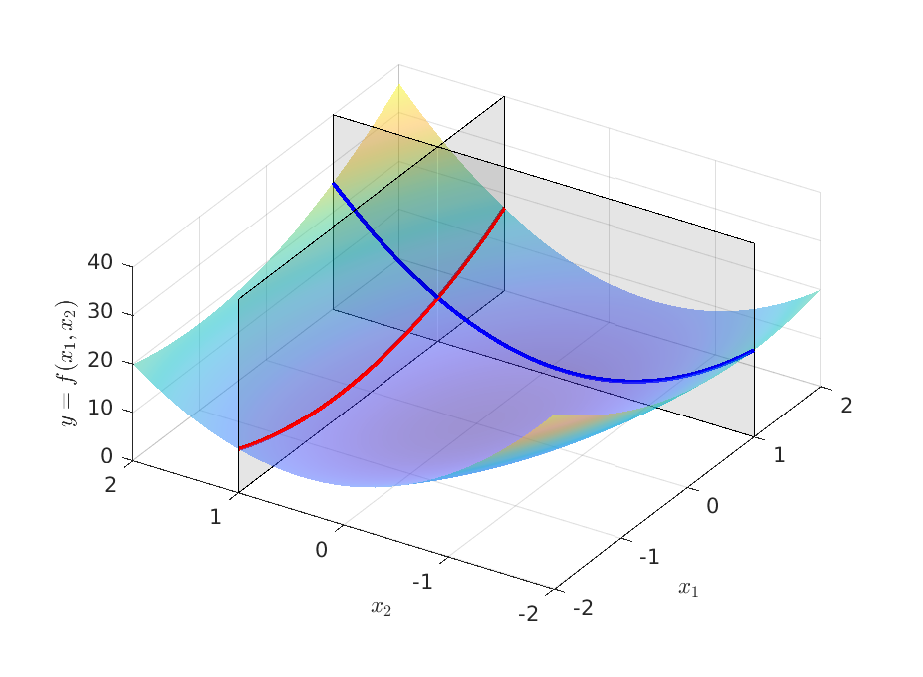
\includegraphics[width=250pt]{chapters/chapter6/figures/fig_motivatingexp.eps}
	\caption{Plot of function $y=f(x_1, x_2)$ in 3-D.} \label{ch6fig_motivatingexp}
\end{figure}

Let $x_2=1$ be constant. Equation \eqref{ch6eq:motivatingexample} becomes
\begin{eqnarray}
	y = f(x_1, 1) = 2x_1^2 + 2x_1 + 1, \nonumber
\end{eqnarray}
which is given by the intersection of  curved surface (equation \eqref{ch6eq:motivatingexample}) and the vertical flat ($x_2=1$) given by the red solid line in Fig. \ref{ch6fig_motivatingexp}. Its derivative with respect to $x_1$ can be easily obtained as
\begin{eqnarray}
	\dfrac{d}{dx_1}f(x_1,1) &=& 4x_1 + 2. \label{ch6eq:motivatingexpdx1}
\end{eqnarray}

Similarly, at $x_1 = 1$, \eqref{ch6eq:motivatingexample} becomes
\begin{eqnarray}
	y = f(1, x_2) = x_2^2 + 2x_2 + 2, \nonumber
\end{eqnarray}
which is given by the blue solid line in Fig. \ref{ch6fig_motivatingexp}. Its derivative with respect to $x_2$ is
\begin{eqnarray}
	\dfrac{d}{dx_2}f(1,x_2) &=& 2x_2 + 2. \label{ch6eq:motivatingexpdx2}
\end{eqnarray}

Consider small vibrations $\Delta x_1$ and $\Delta x_2$. Firstly, let $x_2$ remain constant and only apply $\Delta x_1$ on $y = f(1,1)$. In this case,
\begin{eqnarray}
	\Delta y = f(1+\Delta x_1, 1) - f(1, 1) \approx \dfrac{d}{dx_1}f(x_1,1) \Delta x_1, \label{ch6eq:partialdifx1}
\end{eqnarray}
where $\dfrac{d}{dx_1}f(x_1,1)$ is given in \eqref{ch6eq:motivatingexpdx1}.

On top of \eqref{ch6eq:partialdifx1}, consider vibration $\Delta x_2$. The derivative of function $f(1+\Delta x_1, x_2)$ with respect to $x_2$ depends on $\Delta x_1$ and it is generally unknown without specifying $\Delta x_1$. However, since \eqref{ch6eq:motivatingexample} is continuous and ``smooth'' (Notice that ``smooth'' has specific definition in mathematics. Here, just take its literal meaning: it is perfectly polished without any edges or spikes.), we can intuitively understand that when $\Delta x_1$ is small, $\frac{d}{dx_2}f(1+\Delta x_1, x_2) \approx \frac{d}{dx_2}f(1, x_2)$, and $\frac{d}{dx_2}f(1+\Delta x_1, x_2) \rightarrow \frac{d}{dx_2}f(1, x_2)$ as $\Delta x_1 \rightarrow 0$. Thus, we have
\begin{eqnarray}
	\Delta y &=& \left(f(1+\Delta x_1, 1 + \Delta x_2) -  f(1+\Delta x_1, 1)\right) + \left(f(1+\Delta x_1, 1) - f(1, 1)\right) \nonumber \\
	&\approx& \dfrac{d}{dx_2}f(1,x_2) \Delta x_2 + \dfrac{d}{dx_1}f(x_1,1) \Delta x_1. \label{ch6eq:motivatingresult1}
\end{eqnarray}

In \eqref{ch6eq:motivatingresult1}, consider $\Delta x_1 \rightarrow 0$ and $\Delta x_2 \rightarrow 0$. Denote such $\Delta x_1$ and $\Delta x_2$ as $dx_1$ and $dx_2$ respectively, and the associated $\Delta y$ as $dy$. Here ``$d(\cdot)$'' represents the \textit{infinitesimal change}. Equation \eqref{ch6eq:motivatingresult1} then becomes
\begin{eqnarray}
	d y &=& \dfrac{d}{dx_2}f(1,x_2) d x_2 + \dfrac{d}{dx_1}f(x_1,1) d x_1. \label{ch6eq:motivatingresult2}
\end{eqnarray}

Equation \eqref{ch6eq:motivatingresult2} can be extended to more general cases where $(x_1, x_2) = (1, 1)$ is not specified. The terms $\dfrac{d}{dx_1}f(x_1,1)$ and $\dfrac{d}{dx_2}f(1,x_2)$ needs to be changed accordingly. For example, $\dfrac{d}{dx_1}f(x_1,1)$ given by \eqref{ch6eq:motivatingexpdx1} shall be changed to
\begin{eqnarray}
	\left.\dfrac{d}{dx_1}f(x_1,x_2)\right|_{x_2 \textup{~is constant}} &=& 4x_1 + 2x_2 \nonumber
\end{eqnarray}
with $x_2$ being any arbitrary constant.

The denotation $\left.\dfrac{d}{dx_1}f(x_1,x_2)\right|_{x_2 \textup{~is constant}}$ can sometimes become ambiguous if not handled carefully. One of the reasons could be that ``$d(\cdot)$'' is used as infinitesimal change as shown before. In this case both $dx_1$ and $dx_2$ contribute to $df(x_1,x_2)$, but we would want $\dfrac{d}{dx_1}f(x_1,x_2)$ here to reflect the deviation of $f(x_1,x_2)$ caused by $dx_1$ only, and it is not convenient to list down all the other variables and put ``is/are constant'' everywhere in the equation. Therefore, instead of saying $\left.\dfrac{d}{dx_1}f(x_1,x_2)\right|_{x_2 \textup{~is constant}}$, we denote
\begin{eqnarray}
	\dfrac{\partial}{\partial x_1} f(x_1, x_2) &=& 4x_1 + 2x_2. \nonumber
\end{eqnarray}
The operator $\dfrac{\partial}{\partial x}$ is called \textit{partial derivative} (with respect to $x$), often followed by a multivariable function $f(x,y)$ where $x$ is one of its inputs. It is similar to the derivative, but emphasizing that the interested function is multivariable, and the derivative of this function with respect to ONLY ONE variable is being studied (and the rest variables assumed constant). Since $\partial f(x)$ is rarely or never used as the infinitesimal of $f(x)$, it will hopefully be less ambiguous.

The formal definition of partial derivative is given in next Section \ref{ch6sec:partialtotalderivative}.

Equation \eqref{ch6eq:motivatingresult2} for general $(x_1,x_2)$, therefore, becomes
\begin{eqnarray}
	d y &=& \dfrac{\partial}{\partial x_2}f(x_1,x_2) d x_2 + \dfrac{\partial}{\partial x_1}f(x_1,x_2) d x_1. \label{ch6eq:motivatingtotaldiff}
\end{eqnarray}

The minimum $y=f(x_1,x_2)$ and its associated $x_1$ and $x_2$ can be found by rewriting \eqref{ch6eq:motivatingexample} as
\begin{eqnarray}
	y &=& x_1^2 + \left(x_1 + x_2\right)^2. \nonumber
\end{eqnarray}
Therefore, the minimum $y$ is $y=0$, at $x_1 = 0$ and $x_1 + x_2 = 0$, i.e., $x_1 = x_2 = 0$.

This can also be solved using \eqref{ch6eq:motivatingtotaldiff}. At the minimum point of $y$, $\dfrac{\partial}{\partial x_2}f(x_1,x_2)$ and $\dfrac{\partial}{\partial x_1}f(x_1,x_2)$ must be both zero. Otherwise, it is always possible to add/subtract a small $\Delta x_1$ or $\Delta x_2$ to further decrease $y$. Thus, from \eqref{ch6eq:motivatingexample}
\begin{eqnarray}
	\dfrac{\partial}{\partial x_1}f(x_1,x_2) &=& 4x_1 + 2x_2 = 0 \nonumber \\
	\dfrac{\partial}{\partial x_2}f(x_1,x_2) &=& 2x_1 + 2x_1 = 0 \nonumber
\end{eqnarray}
which yields $x_1=x_2=0$.

\section{Partial Derivative} \label{ch6sec:partialtotalderivative}

In the case of single input scalar function $f(x), x \in \mathbb{R}$, there is no point to define partial and total derivative, as the derivative with respect to that single variable by itself is the total derivative.

In the case of multivariable function with multiple inputs, $f(x), x \in \mathbb{R}^{R\times 1}$, the definition partial derivative is given below.

\begin{VF}
	\textbf{Definition of Partial Integral}:
	\\
	\\
	Consider function $y = f(x_1,...,x_n)$ where $y$ is the scalar output and $x = \left[x_1, ..., x_n\right]^T$ is a $n\times 1$ vector input. The partial derivative of $y=f(x)$ with respect to $x_i$ is given by
	\begin{eqnarray}
		\dfrac{\partial}{\partial x_i}f(x) = \lim_{\Delta x_i \rightarrow 0} \dfrac{f(x_1,..., x_i + \Delta x_i,...,x_n)-f(x_1,...,x_n)}{\Delta x_i}, \label{ch6eq:formalpartialderivative}
	\end{eqnarray}
	with $x_1,...,x_{i-1}, x_{i+1},..., x_n$ remaining constant, and only $x_i$ is allowed to vary.
	
\end{VF}

Here is another example to help better understand partial derivative. Consider $z=f(x, y)$ a multivariable function of both inputs $x$, $y$ as follows
\begin{eqnarray}
	z = f(x,y) = x^2 + \textup{sin}(y), \label{ch6eq:partialdiffchainexp1}
\end{eqnarray}
where $y = g(x)$ is a single input function of $x$ as follows
\begin{eqnarray}
	y = g(x) = e^x. \label{ch6eq:partialdiffchainexp2}
\end{eqnarray}

Apparently, the value of $z$ ultimately depends on $x$ alone, but in the intermediate calculation, $z$ depends on both $x$ and $y$. The calculation flow is visualized in Fig. \ref{ch6fig_chainexp}.

\begin{figure}
	\centering
	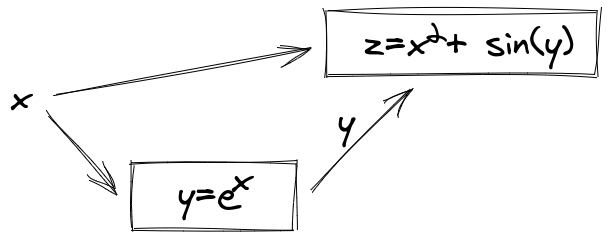
\includegraphics[width=200pt]{chapters/chapter6/figures/chainexp.png}
	\caption{The calculation of $z$ using $x$ and $y$.} \label{ch6fig_chainexp}
\end{figure}

In this case, the total derivative $\dfrac{d}{dx}f(x, y)$ can be expressed as follows
\begin{eqnarray}
	\dfrac{d}{dx}f(x, y) &=& \dfrac{\partial}{\partial x} f(x, y) + \dfrac{\partial}{\partial y}f(x, y) \dfrac{d}{dx}y. \label{ch6eq:partialvstotal}
\end{eqnarray}
where in this example,
\begin{eqnarray}
	\dfrac{\partial}{\partial x} f(x, y) &=& 2x \nonumber \\
	\dfrac{\partial}{\partial y} f(x, y) &=& \textup{cos}(y) \nonumber \\
	\dfrac{d}{dx}y &=& e^x \nonumber
\end{eqnarray}
and finally
\begin{eqnarray}
	\dfrac{d}{dx}f(x, y) &=& 2x + \textup{cos}(e^x)e^x \nonumber
\end{eqnarray}

Sometimes \eqref{ch6eq:partialvstotal} is rewritten as follows
\begin{eqnarray}
	df(x, y) &=& \dfrac{\partial}{\partial x} f(x, y) dx + \dfrac{\partial}{\partial y}f(x, y) dy \nonumber \\
	dy &=& \left(\dfrac{d}{dx}y\right) dx \nonumber
\end{eqnarray}
where $d(\cdot)$ represents the infinitesimal change of a variable.

Equation \eqref{ch6eq:partialvstotal} serves as a good example to show the relationship and difference between the total derivative $\dfrac{d}{dx}f(x, y)$ and the partial derivative $\dfrac{\partial}{\partial x} f(x, y)$. When calculating total derivative, all variables that would affect the value of the function must be taken into consideration, while when calculating partial derivative, only one input variable is studied, with the rest variables remaining constant.

For a function with $1$ output and $n$ inputs, sometimes it is convenient to put the partial derivative to each input in a vector. For example, for $y=f(x)$ where $x = \left[x_1,...,x_n\right]^T$, denote
\begin{eqnarray}
	\dfrac{\partial}{\partial x}f(x) = \left[\begin{array}{ccc}
	\dfrac{\partial}{\partial x_1}f(x) &
	\ldots &
	\dfrac{\partial}{\partial x_n}f(x)
	\end{array}\right] \label{ch6eq:scalarbyvector}
\end{eqnarray}
as the \textit{scalar-by-vector derivative}. Notice that \eqref{ch6eq:scalarbyvector} is usually given as a row vector. In some research papers the result is given as a column vector, i.e. the transpose of \eqref{ch6eq:scalarbyvector}.

For a function with $m$ outputs and $1$ input $y=f(x)$ where $y = \left[y_1,...,y_m\right]^T = \left[f_1(x),...,f_m(x)\right]^T$, its \textit{vector-by-scalar derivative} is given by
\begin{eqnarray}
	\dfrac{\partial}{\partial x}f(x) &=& \left[\begin{array}{c}
	\dfrac{\partial}{\partial x}f_1(x) \\
	\vdots \\
	\dfrac{\partial}{\partial x}f_m(x)
	\end{array}\right]. \label{ch6eq:vectorbyscalar}
\end{eqnarray}

And finally for a function with $m$ outputs and $n$ inputs $y=f(x)$ where $y = \left[y_1,...,y_m\right]^T = \left[f_1(x),...,f_m(x)\right]^T$ and $x = \left[x_1,...,x_n\right]^T$, the \textit{vector-by-vector} derivative is given by
\begin{eqnarray}
	\dfrac{\partial}{\partial x}f(x) &=& \left[\begin{array}{ccc}
	\dfrac{\partial}{\partial x_1}f_1(x) & \ldots & \dfrac{\partial}{\partial x_n}f_1(x) \\
	\vdots & \ddots & \vdots \\
	\dfrac{\partial}{\partial x_1}f_m(x) & \ldots & \dfrac{\partial}{\partial x_n}f_m(x) \\
	\end{array}\right]. \label{ch6eq:vectorbyvector}
\end{eqnarray}

Partial derivative and the above equations \eqref{ch6eq:scalarbyvector}, \eqref{ch6eq:vectorbyscalar} and \eqref{ch6eq:vectorbyvector} have many applications. Two of those most popular use cases are \textit{gradient} and \textit{Jacobian matrix}. Since they are so important and widely used, it is worth especially introducing them in specific Sections \ref{ch6sec:gradient} and \ref{ch6sec:jacobianmatrix}.

\section{Gradient} \label{ch6sec:gradient}

For a scalar-valued multivariable function $y=f(x)$ where $y$ is a scalar and $x$ is a vector $x = \left[\begin{array}{ccc}
                                                                               x_1 & \ldots & x_n
                                                                             \end{array}\right]^T \in \mathbb{R}^n$, the gradient studies the ``direction'' of $\Delta x$ in $\mathbb{R}^n$ space that causes $y$ to increase/decrease the fastest.

The gradient of such function $f(x)$ is a vector function of $x$, denoted by $\nabla f(x)$. Notice that $\nabla f(x) \in \mathbb{R}^n$ is a vector in the same space with $x$, since it indicates a ``direction'' of $x$.

Section \ref{ch6subsec:gradientmotivatingexp} gives a motivating example of gradient, and Section \ref{ch6subsec:gradientdef} gives its formal definition.

\subsection{Motivating Example} \label{ch6subsec:gradientmotivatingexp}

The following motivating example helps to illustrate the calculation and use case of gradient.

\begin{shortbox}
\Boxhead{A Motivating Example}

Consider the following function $y=f(x)$ where $x = [x_1,x_2]^T$ is a vector and
\begin{eqnarray}
    y = f(x) = 2\textup{sin}(x_1) + \textup{sin}\left(\dfrac{x_1}{2} + \pi\right) + \textup{sin}(2x_2) \label{ch6eq:gradientexp_hill}
\end{eqnarray}
where $x_1\in[-3,3]$ and $x_2\in[-2,2]$. The 3-D plot and the contour line of the function are given in Figs \ref{ch6fig:gradientexp_3d} and \ref{ch6fig:gradientexp_contour} respectively.

%The objective is to obtain such $x_1$ and $x_2$ to maximize $y$. By applying a glomal optimization on \eqref{ch6eq:gradientexp_hill}, $x_1 = 1.3764$, $x_2=0.7854$ can be obtained. However, in this example we are assuming that the global optimization is not applicable due to the lack of information or computational power. Try to obtain the target coordinate $x_1$ and $x_2$ without using global optimization.

Consider initial point $x^0 = [x_1^0, x_2^0]^T = [1,0]^T$. Let $x$ deviate a little bit from $x^0$ to get $x^1 = [x_1^1, x_2^1]^T = [x_1^0 + \Delta x_1^0, x_2^0 + \Delta x_2^0]^T$. The objective is to find such $\Delta x^0 = [\Delta x_1^0, \Delta x_2^0]^T$ to hopefully get $f(x^1)$ as large as possible.

\end{shortbox}

\begin{figure}
	\centering
	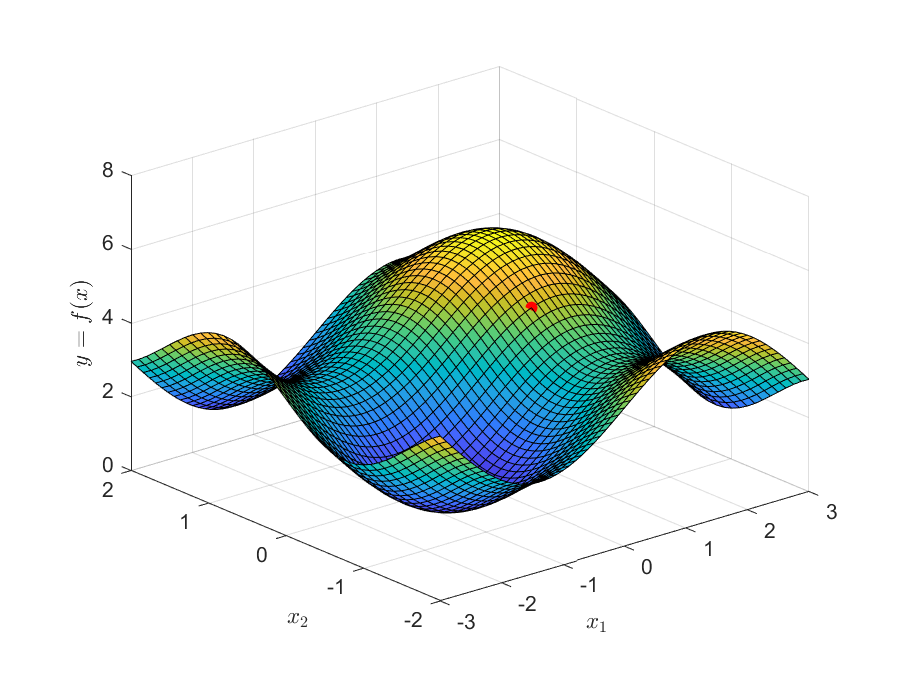
\includegraphics[width=250pt]{chapters/chapter6/figures/gradientexp_3d.eps}
	\caption{Plot of $y=f(x_1, x_2)$ in 3-D.} \label{ch6fig:gradientexp_3d}
\end{figure}
\begin{figure}
	\centering
	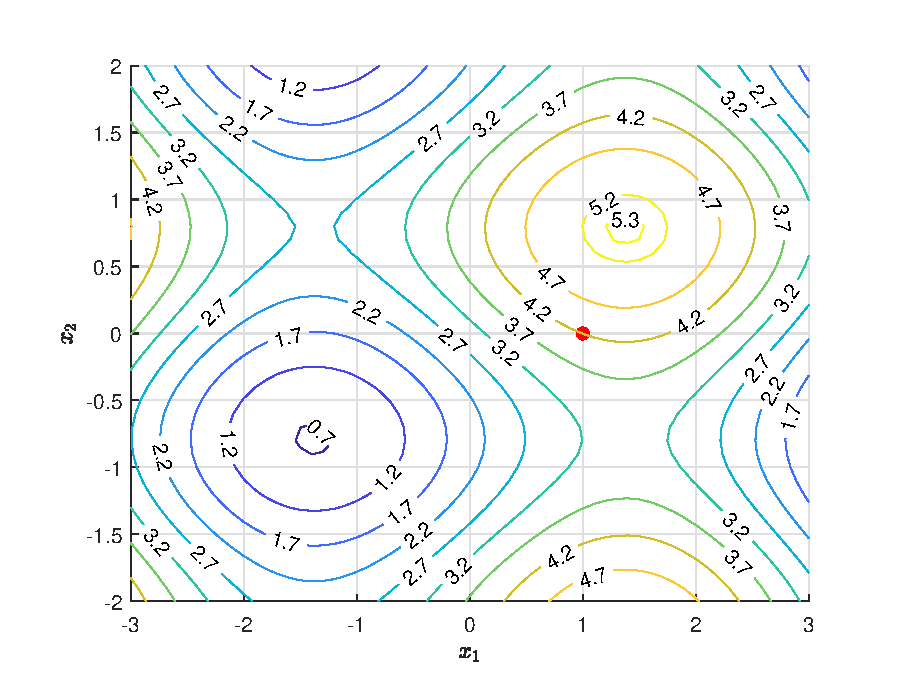
\includegraphics[width=250pt]{chapters/chapter6/figures/gradientexp_contour.eps}
	\caption{Contour line of $y=f(x_1, x_2)$.} \label{ch6fig:gradientexp_contour}
\end{figure}

Notice that $\Delta x^0$ can be interpreted as a vector that indicates the ``direction'', along which trace the value of $y$ increases the fastest. An intuitive way is to find the tangent plane to the surface at $x=[1,0]^T$, and let $\Delta x^0$ be the direction where it climbs up the tangent plane the fastest. 

From space analytic geometry, we know that a pair of unparalleled vector can uniquely define a plane, and such pair of vector is not difficult to find, as
\begin{eqnarray}
 \vec{v}_1 &=& \left(\begin{array}{ccc}
                       1, & 0, & \left.\dfrac{\partial y}{\partial x_1}\right|_{x=x^0}
                     \end{array}\right) \label{ch6eq:gradientexp_v1} \\
 \vec{v}_2 &=& \left(\begin{array}{ccc}
                       0, & 1, & \left.\dfrac{\partial y}{\partial x_2}\right|_{x=x^0}
                     \end{array}\right) \label{ch6eq:gradientexp_v2}
\end{eqnarray}
must be such a pair of vector. This is because \eqref{ch6eq:gradientexp_v1} is the tangent of the 2-D intersect of $y=f(x_1,x_2)$ and $x_2 = x_2^k$ (i.e. $y=f(x_1,x_2^k)$), therefore must be tangent to the original 3-D surface $y=f(x_1,x_2)$. The same applies to \eqref{ch6eq:gradientexp_v2}, making it also tangent to $y=f(x_1,x_2)$. And obviously the two lines are unparalleled since one of them lies on plane $x_1=x_1^k$ and the other on plane $x_2=x_2^k$, which are two perpendicular planes.

At $x^0=[1,0]$, the intersect of $y=f(x_1,x_2)$ and $x_2 = 0$ is given as the red solid line in Fig. \ref{ch6fig:gradientexp_3d2}, and its tangent at $\left(1,0,f(1,0)\right)$, i.e. equation \eqref{ch6eq:gradientexp_v1}, is given by the red dashed line. The same is applied for the intersect of $y=f(x_1,x_2)$ and $x_1 = 1$ and its tangent equation \eqref{ch6eq:gradientexp_v2} as the blue lines.

\begin{figure}
	\centering
	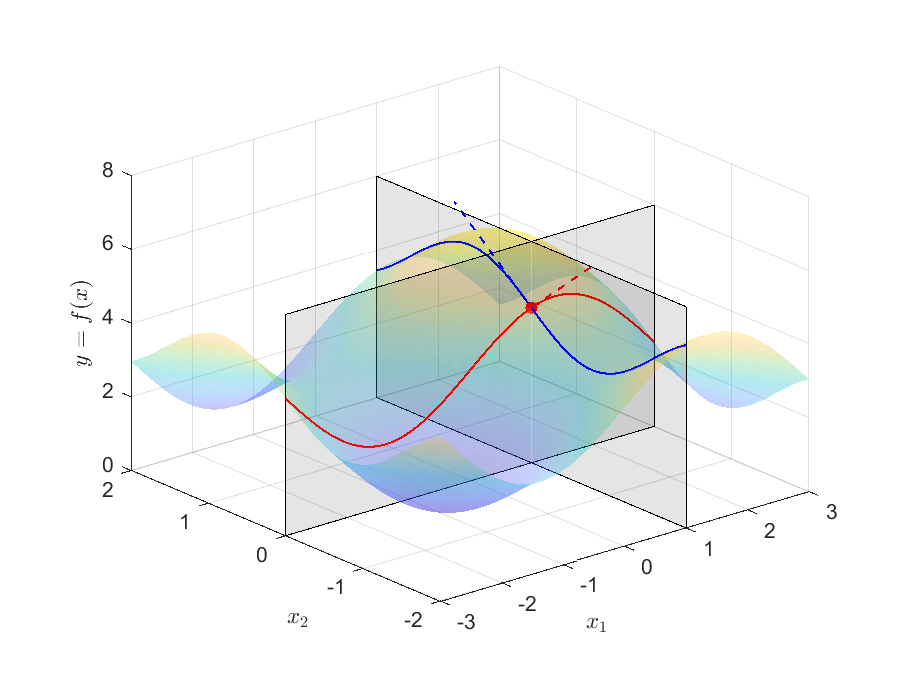
\includegraphics[width=250pt]{chapters/chapter6/figures/gradientexp_3d2.eps}
	\caption{Plot of vectors given by \eqref{ch6eq:gradientexp_v1} and \eqref{ch6eq:gradientexp_v2}.} \label{ch6fig:gradientexp_3d2}
\end{figure}

The two vectors \eqref{ch6eq:gradientexp_v1} and \eqref{ch6eq:gradientexp_v2}, as indicated by the red and blue dashed lines respectively in Fig. \ref{ch6fig:gradientexp_3d2} are unparalleled and intersect at $\left(1,0,f(1,0)\right)$. Therefore, the vectors can uniquely determine a plane which is the tangent plan for $y=f(x_1,x_2)$ at $\left(1,0,f(1,0)\right)$, as shown by Fig. \ref{ch6fig:gradientexp_3d3}.

\begin{figure}
	\centering
	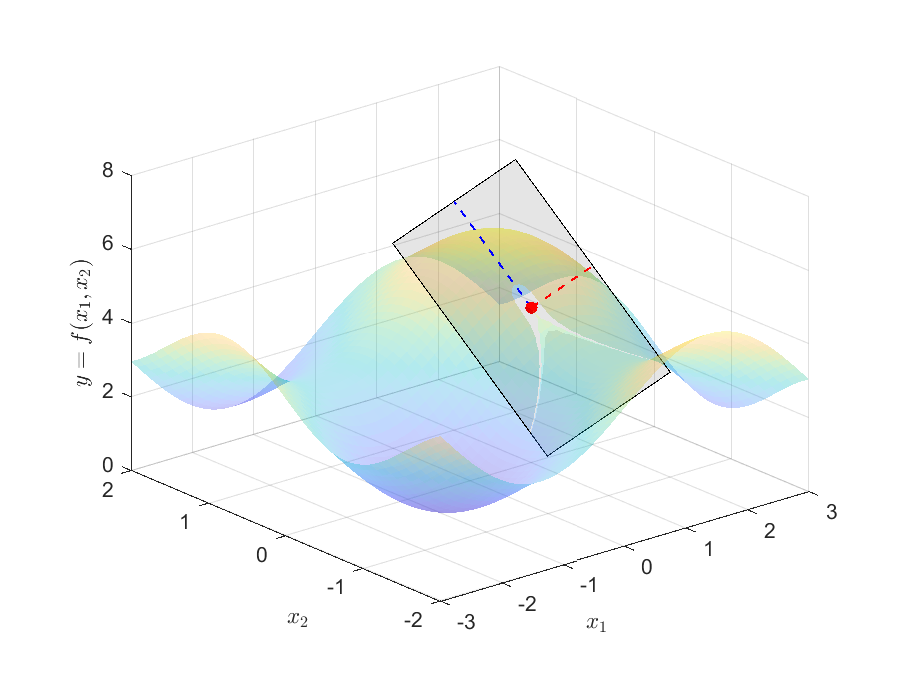
\includegraphics[width=250pt]{chapters/chapter6/figures/gradientexp_3d3.eps}
	\caption{Formulation of the tangent plane from vectors given by \eqref{ch6eq:gradientexp_v1} and \eqref{ch6eq:gradientexp_v2}.} \label{ch6fig:gradientexp_3d3}
\end{figure}

The next step is to find a vector $\vec{v}$ on the tangent plane along which $y$ increases the fastest. The direction of this vector will be used as a guidance in selecting $\Delta x^k = [\Delta x_1^k, \Delta x_2^k]$. This vector can be derived using space analytic geometry and it is briefly introduced as follows.

For convenience, we will do a plane transformation to the tangent plane so that it crosses the origin $(0,0,0)$. This can be done by mapping $\left(x_1^k,x_2^k,f(x_1^k,x_2^k)\right)$ to $(0,0,0)$. The vector $\vec{v}$ must fulfill the following two conditions: (a) it must be on the tangent plane; (b) it must be perpendicular to the intersection line of the tangent plane and the $y=0$ plane.

Consider (a). Since the vector is on the tangent plan, it can be represented as a linear combination of \eqref{ch6eq:gradientexp_v1} and \eqref{ch6eq:gradientexp_v2} as
\begin{eqnarray}
    \vec{v}&=& \left(\begin{array}{ccc}
              \lambda_1, & \lambda_2, & \lambda_1\left.\dfrac{\partial y}{\partial x_1}\right|_{x=x^k} + \lambda_2\left.\dfrac{\partial y}{\partial x_2}\right|_{x=x^k}
            \end{array} \right) . \label{ch6eq:gradient_v}
\end{eqnarray}

Consider (b). The analytical expression for the tangent plane can be obtained by calculating its normal vector as follows.
\begin{eqnarray}
  \vec{n} &=& \vec{v}_1 \times \vec{v}_2 \nonumber \\
  &=& \left(\begin{array}{ccc}
              -\left.\dfrac{\partial y}{\partial x_1}\right|_{x=x^k}, & -\left.\dfrac{\partial y}{\partial x_2}\right|_{x=x^k}, & 1
            \end{array}\right) \nonumber
\end{eqnarray}
Therefore, the tangent plan is given by (cross origin $(0,0,0)$)
\begin{eqnarray}
  y &=& \left.\dfrac{\partial y}{\partial x_1}\right|_{x=x^k} x_1 + \left.\dfrac{\partial y}{\partial x_2}\right|_{x=x^k} x_2 \nonumber
\end{eqnarray}
And its intersection with plane $y=0$ is
\begin{eqnarray}
  \left.\dfrac{\partial y}{\partial x_1}\right|_{x=x^k} x_1 + \left.\dfrac{\partial y}{\partial x_2}\right|_{x=x^k} x_2 &=& 0 \label{ch6eq:gradient_intersectline}
\end{eqnarray}
Vector $\vec{v}$ must be perpendicular to \eqref{ch6eq:gradient_intersectline}. A quick way is to pick a vector from \eqref{ch6eq:gradient_intersectline}, for example,
\begin{eqnarray}
   \vec{v}_{\textup{intersect}} &=& \left(\begin{array}{ccc}
              \left.\dfrac{\partial y}{\partial x_2}\right|_{x=x^k}, & -\left.\dfrac{\partial y}{\partial x_1}\right|_{x=x^k}, & 0
            \end{array}\right), \label{ch6eq:gradient_intersectvector}
\end{eqnarray}
and make sure $\vec{v}_{\textup{intersect}}$ is perpendicular to $\vec{v}$. From \eqref{ch6eq:gradient_v} and \eqref{ch6eq:gradient_intersectvector}, equating $\vec{v} \cdot \vec{v}_{\textup{intersect}} = 0$ gives
\begin{eqnarray}
  \lambda_1 \left.\dfrac{\partial y}{\partial x_2}\right|_{x=x^k} &=& \lambda_2 \left.\dfrac{\partial y}{\partial x_1}\right|_{x=x^k} \label{ch6eq:gradient_lambdarestrict}
\end{eqnarray}

Equation \eqref{ch6eq:gradient_lambdarestrict} has infinite number of solutions, all of which result in the same direction of $\vec{v}$. For example, select $\lambda_1 = \left.\dfrac{\partial y}{\partial x_1}\right|_{x=x^k}$, $\lambda_2 = \left.\dfrac{\partial y}{\partial x_2}\right|_{x=x^k}$. Substituting $\lambda_1$ and $\lambda_2$ into \eqref{ch6eq:gradient_v} gives
\begin{eqnarray}
  \vec{v} &=& \left(\begin{array}{cc}
              \left.\dfrac{\partial y}{\partial x_1}\right|_{x=x^k}, & \left.\dfrac{\partial y}{\partial x_2}\right|_{x=x^k},
            \end{array} \right. \nonumber \\
            && \left. \left.\dfrac{\partial y}{\partial x_1}\right|_{x=x^k} \left.\dfrac{\partial y}{\partial x_1}\right|_{x=x^k} + \left.\dfrac{\partial y}{\partial x_2}\right|_{x=x^k} \left.\dfrac{\partial y}{\partial x_2}\right|_{x=x^k} \right). \label{ch6eq:gradient_finalv}
\end{eqnarray}

Equation \eqref{ch6eq:gradient_finalv} gives the guidance of the direction from $x^k$ to $x^{k+1}$ which can hopefully maximize $f(x_1^{k+1}, x_2^{k+1})$. Therefore, $\Delta x^k$ can be obtained as follows.
\begin{eqnarray}
  \Delta x^k &=& \left[\begin{array}{cc}
                         \Delta x_1^k & \Delta x_2^k
                       \end{array}\right]^T \nonumber \\
  &=& \alpha \left[\begin{array}{c}
                         \left.\dfrac{\partial y}{\partial x_1}\right|_{x=x^k} \\
                         \left.\dfrac{\partial y}{\partial x_2}\right|_{x=x^k}
                       \end{array}\right] \nonumber \\
  &=& \alpha \left.\nabla f(x)\right|_{x=x^k}
\end{eqnarray}
where $\alpha > 0$ is an adjustable parameter to determine the progressing rate for each iteration and
\begin{eqnarray}
  \nabla f(x) &=& \left[\begin{array}{c}
                         \dfrac{\partial y}{\partial x_1} \\
                         \dfrac{\partial y}{\partial x_2}
                       \end{array}\right] \label{ch6eq:gradientdef}
\end{eqnarray}  
is defined as the \textit{gradient} of $f(x)$, which by itself is a vector function of $x$.
















\subsection{Gradient of a Multivariable Function} \label{ch6subsec:gradientdef}




\section{Jacobian Matrix} \label{ch6sec:jacobianmatrix}


\part{Linux Advanced}

% Linux admin basics
\chapter{Multiple Integral} \label{ch7ch}

The integral for scalar input function has been introduced in Chapter \ref{ch3}. The integral of $y=f(x)$ with the lower bound $a$ and upper bound $b$ is denoted by \eqref{ch3eq:generaldefiniteintegral2}. It is defined as the limit of sum given by \eqref{ch3eq:generaldefiniteintegral}, and can be interpreted as the area circulated by $x=a$, $x=b$, $y=f(x)$ and $y=0$ as shown by Fig. \ref{ch3fig:explainintegrial}. In practice, the integral can be calculated using \eqref{ch3eq:calculatedefiniteintegral}.

In this chapter, the integral for multiple input functions is introduced. Motivating examples are used to illustrate the basic concept and meaning of multiple integral in Section \ref{ch7sec:motivatingexp}. The formal definition of multiple integral is given in Section \ref{ch7sec:multipleintegral}.

\section{Motivating Examples} \label{ch7sec:motivatingexp}

\begin{shortbox}
\Boxhead{Motivating Example 1}

Consider calculating the volume of a cone using integral. The bottom radius and the height of the cone are $1$ and $3$ respectively.

\end{shortbox}

Figure \ref{ch7fig:motivatingexp1} gives a demonstration of the cone in the motivating example. Using similar ideas introduced in Chapter \ref{ch3}, we know that we can think of the cone as a combination of thin cylinders, whose radiuses depend on the vertical position ($z$-axis position) of the associated cylinder. For example, at $z=1.5$, the radius of the cylinder is $0.5$.

\begin{figure}
	\centering
	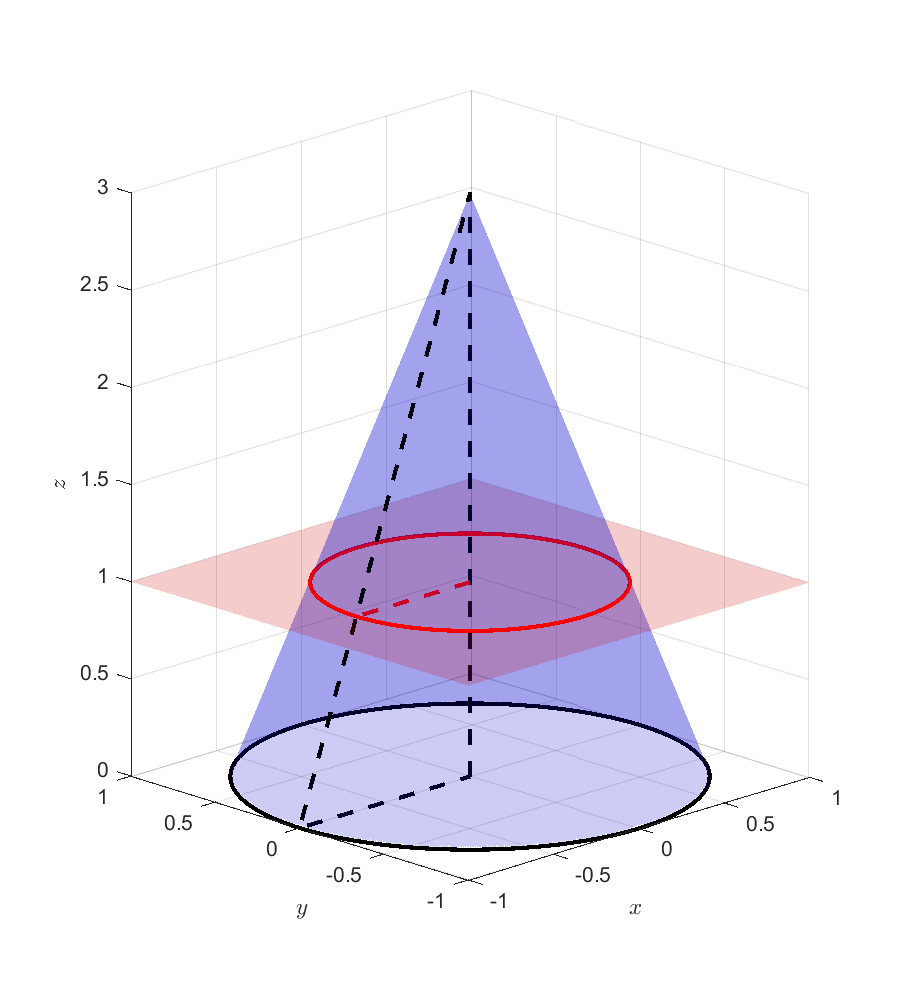
\includegraphics[width=200pt]{chapters/chapter7/figures/motivatingexp1.eps}
	\caption{Calculation of the volume of a cone.} \label{ch7fig:motivatingexp1}
\end{figure}

The volume of the cone can be obtained by letting the thickness of each cylinder approaches zero. i.e.,
\begin{eqnarray}
  V &=& \int_{0}^{3}S(z)dz, \label{ch7eq:motivatingv} \\
  S(z) &=& \pi R(z)^2, \label{ch7eq:motivatingsz} \\
  R(z) &=& \dfrac{3-z}{3}, 0\leq z\leq 3, \label{ch7eq:motivatingrz}
\end{eqnarray}
where $R(z)$ and $S(z)$ are the bottom circle radius and area of the thin cylinder at vertical position $z$, and $S(z)dz$ can be interpreted as the volume of this thin cylinder.

Substituting \eqref{ch7eq:motivatingsz} and \eqref{ch7eq:motivatingrz} into \eqref{ch7eq:motivatingv} gives
\begin{eqnarray}
  V = \int_{0}^{3} \dfrac{\pi}{9} \left(3-z\right)^2 dz
  = \left.\dfrac{\pi}{27}(z-3)^3 \right|_0^3
  = \pi, \nonumber
\end{eqnarray}
which is consistent with what we learned in primary school: the volume of a cone is one third of its bottom area multiplied by its height.

The above motivating example 1 implies the volume of an object might be formulated as an one-dimensional integration. As a first step, a direction, such as $z$-axis as given in the motivating example 1, is chosen. Next, imagine using planes to intersect the object. Each plane shall be perpendicular to the selected direction, as given by the red plane in Fig. \ref{ch7fig:motivatingexp1}. Notice that the red plane is perpendicular to the direction of $z$-axis. The intersection area shall be a function of the intersection position, as given by \eqref{ch7eq:motivatingsz}. Finally, the volume can be calculated as the integral of the area function over the direction, as given by \eqref{ch7eq:motivatingv}.

In many cases, the calculation of the intersection area can be less simple and intuitive than \eqref{ch7eq:motivatingsz}. An example is given by the following motivating example.

\begin{shortbox}
	\Boxhead{Motivating Example 2}
	
	Consider calculating the volume surrounded by the following surfaces:
	\begin{eqnarray}
		0\leq &x& \leq 2\pi, \nonumber \\
		0\leq &y& \leq 2\pi, \nonumber \\
		0\leq &z& \leq f(x,y) = y\textup{cos}(x+y)+2\pi. \label{ch7eq:motivatingexp2f}
	\end{eqnarray}
	
\end{shortbox}

We will use the same method adopted from the motivating example 1 to solve motivating example 2. The volume to be calculated is plotted in Fig. \ref{ch7fig:motivatingexp2} (only the top surface). The $x$-axis direction is chosen for the integral in motivating example 2.

It can be spotted soon that motivating example 2 is more complicated than 1 as the intersection area, in this case $S(x)$ as a function of position $x$, cannot be obtained as intuitively as \eqref{ch7eq:motivatingsz}.

As an example for illustration, in Fig. \ref{ch7fig:motivatingexp2} the red surface is the intersection surface at $x=2$, and $S(x)$ at $x=2$ should be the area surrounded by the red line. At a first glance, it seems that $S(x)$ does not have an analytical expression as the red line shape is quite arbitrary.

\begin{figure}
	\centering
	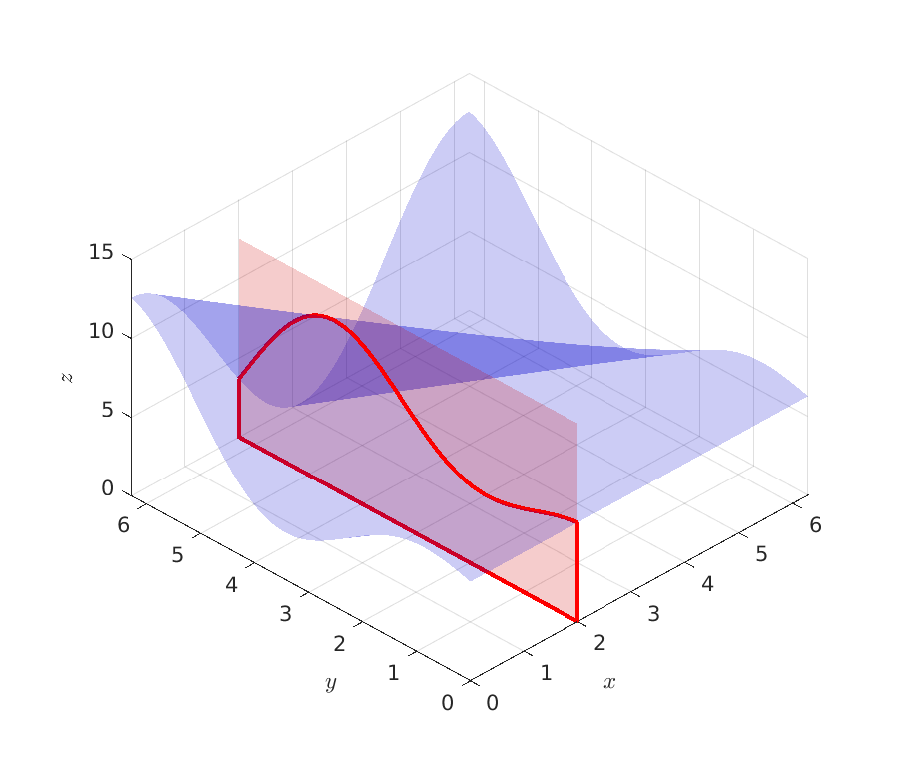
\includegraphics[width=200pt]{chapters/chapter7/figures/motivatingexp2.eps}
	\caption{Calculation of volume of an arbitrary arbitrary project.} \label{ch7fig:motivatingexp2}
\end{figure}

However, this is not true. The area surrounded by the red line in Fig. \ref{ch7fig:motivatingexp2} can be calculated with the knowledge introduced in Chapter \ref{ch3} as follows. Substituting constant $x=2$ into \eqref{ch7eq:motivatingexp2f} gives
\begin{eqnarray}
	z = f(2,y) = y\textup{cos}(y+2) + 2\pi, 0\leq y\leq2\pi, \nonumber
\end{eqnarray}
which is the analytical expression of the red line (intersecting with the top surface). Therefore, the corresponding area in Fig. \ref{ch7fig:motivatingexp2} is
\begin{eqnarray}
	S(x)|_{x=2} &=& \int_{0}^{2\pi} f(2,y) dy \nonumber \\ &=& \int_{0}^{2\pi}\left(y\textup{cos}(y+2) + 2\pi\right)dy \nonumber \\
	&=& \left.\left(y\textup{sin}(y+2)+\textup{cos}(y+2) + 2\pi y\right)\right|_{0}^{2\pi} \nonumber \\
	&=& 2\pi\textup{sin}(2) + 4\pi^2. \nonumber
\end{eqnarray}

Without specifying $x$ as any particular value, $S(x)$ is in general given by
\begin{eqnarray}
	S(x) &=& \int_{0}^{2\pi} f(x,y) dy \label{ch7eq:motivatingexp2sx0} \\ &=& \int_{0}^{2\pi}\left(y\textup{cos}(x+y)+2\pi\right)dy \label{ch7eq:motivatingexp2sx} \\
	&=& \left.\left(y\textup{sin}(x+y)+\textup{cos}(x+y) + 2\pi y\right)\right|_{0}^{2\pi} \label{ch7eq:motivatingexp2sx2} \\
	&=& 2\pi\textup{sin}(x) + 4\pi^2, \label{ch7eq:motivatingexp2sx3}
\end{eqnarray}
where \eqref{ch7eq:motivatingexp2sx2} is derived from \eqref{ch7eq:motivatingexp2sx} by treating $x$ as a constant value. Using  \eqref{ch7eq:motivatingexp2sx0} and \eqref{ch7eq:motivatingexp2sx3}, the volume in motivating example 2 can be calculated as
\begin{eqnarray}
	V &=& \int_{0}^{2\pi} S(x) dx \nonumber \\
	&=& \int_{0}^{2\pi} \left[\int_{0}^{2\pi}f(x,y)dy\right]dx \label{ch7eq:motivatingexp2doubleintegral} \\
	&=& \int_{0}^{2\pi} \left[ \int_{0}^{2\pi}\left(y\textup{cos}(x+y)+2\pi\right)dy\right] dx \nonumber \\
	&=& \int_{0}^{2\pi} \left(2\pi\textup{sin}(x) + 4\pi^2\right) dx \nonumber \\
	&=& \left.\left(-2\pi\textup{cos}(x) + 4\pi^2 x\right)\right|_{0}^{2\pi} \nonumber \\
	&=& 8\pi^3. \nonumber
\end{eqnarray}

In \eqref{ch7eq:motivatingexp2doubleintegral}, two integrals are calculated one after another to finally obtain the volume of motivating example 2. There is an alternative way of understanding \eqref{ch7eq:motivatingexp2doubleintegral} that gives more insights to the problem. From \ref{ch3}, we know that $dx$ and $dy$ are the infinitesimal change along $x$-axis and $y$-axis respectively, and the two-step integrals are essentially the calculation of infinite sum of $f(x,y)$ multiplied by $\Delta x$ and $\Delta y$ as given in the equation below, with $\Delta x, \Delta y \rightarrow 0$. To conclude, \eqref{ch7eq:motivatingexp2doubleintegral} can be rewritten as
\begin{eqnarray}
  \int_{0}^{2\pi} \left[\int_{0}^{2\pi}f(x,y)dy\right]dx &=& \lim_{\Delta x, \Delta y \rightarrow 0} \sum_{i} \left[\sum_{j} f(x_{i},y_{j}) \Delta y \right] \Delta x \nonumber \\
  &=& \lim_{\Delta x, \Delta y \rightarrow 0} \sum_{i,j} f(x_i,y_j) \Delta x \Delta y, \label{ch7eq:motivatingexp2deltaxy}
\end{eqnarray}
where \eqref{ch7eq:motivatingexp2deltaxy} represents the sum of a volume of cubes with the bottom area $\Delta x \times \Delta y$ and different height $f(x_i,y_j)$, as demonstrated by Fig. \ref{ch7fig:motivatingexp2p2}. With $\Delta x, \Delta y \rightarrow 0$, the precise volume of the arbitrary object can be obtained.

\begin{figure}
	\centering
	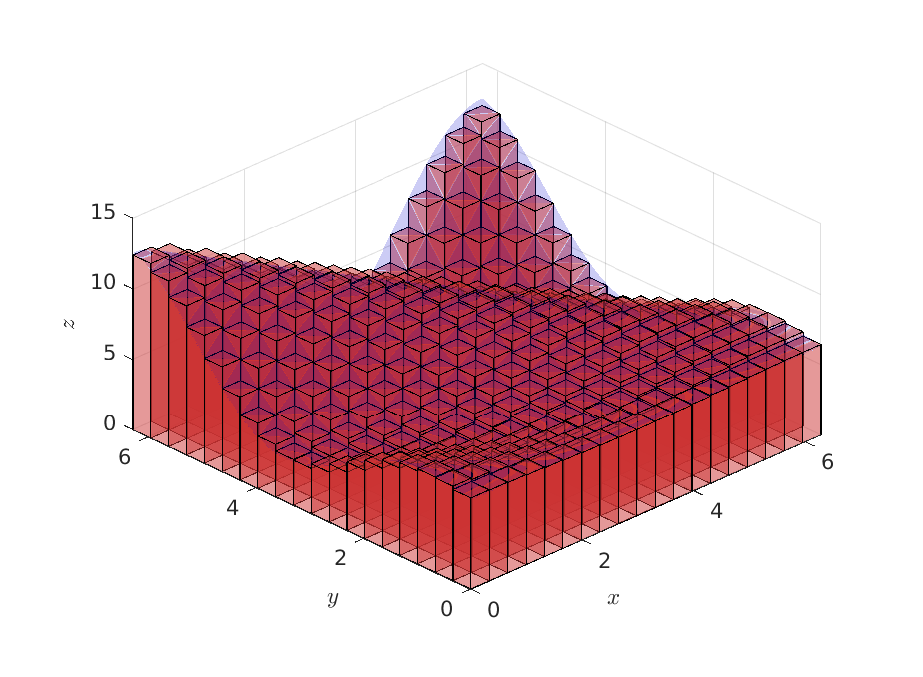
\includegraphics[width=200pt]{chapters/chapter7/figures/motivatingexp2p2.eps}
	\caption{Calculation of volume of an arbitrary object as sum of cubes.} \label{ch7fig:motivatingexp2p2}
\end{figure}

Notice that as long as \eqref{ch7eq:motivatingexp2deltaxy} exists, the sequence of the summation is irrelevant to the result. For example, the cubes with the same $x$-axis position can be added together first (as demonstrated by the red cubes in Fig. \ref{ch7fig:motivatingexp2p3}). Then the sum of volume of cubes at different $x$-axis positions are added together. Similarly, it can be done in the other way around. The cubes with the same $y$-axis position can be added together first (as demonstrated by the green cubes in Fig. \ref{ch7fig:motivatingexp2p3}).

\begin{figure}
	\centering
	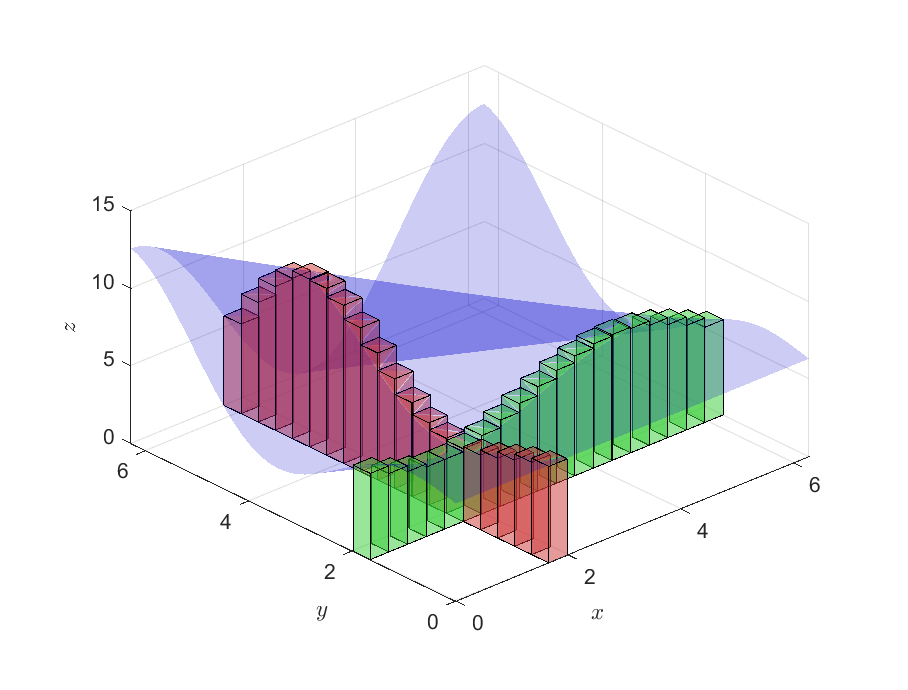
\includegraphics[width=200pt]{chapters/chapter7/figures/motivatingexp2p3.eps}
	\caption{Summation of cubes in different sequence.} \label{ch7fig:motivatingexp2p3}
\end{figure}

Equation \eqref{ch7eq:motivatingexp2deltaxy} is denoted by
\begin{eqnarray}
  \lim_{\Delta x, \Delta y \rightarrow 0} \sum_{i,j} f(x_i,y_j) \Delta x \Delta y &=& \int_{0}^{2\pi}\int_{0}^{2\pi} f(x,y) dx dy ,\label{ch7eq:motivatingexp2def}
\end{eqnarray}
which is an example of double integral. And in this example, we already know that to solve \eqref{ch7eq:motivatingexp2def}, we can use either \eqref{ch7eq:motivatingexp2doubleintegral} or
\begin{eqnarray}
  \int_{0}^{2\pi}\int_{0}^{2\pi} f(x,y) dx dy &=& \int_{0}^{2\pi} \left[\int_{0}^{2\pi}f(x,y)dx\right]dy, \nonumber
\end{eqnarray}
both shall give the same result as the sequence of integral over $x$ or $y$ is irrelevant as long as \eqref{ch7eq:motivatingexp2def} exists. Notice that for multiple integral sometimes $\iint$, $\iiint$, etc., symbols are used for simplicity when the upper and lower boundary of the integral variables are the same or not given in the equation. Thus, \eqref{ch7eq:motivatingexp2def} can also be written as $\iint_{0}^{2\pi} f(x,y)dx dy$.

\section{Multiple Integral} \label{ch7sec:multipleintegral}

The definition of double integral is given below. Higher order of integral can be achieved by expanding the double integral into a higher dimension hyperspace.

\begin{VF}
    \textbf{Definition of Double Integral}:
    \\
    \\
Given a function $f(x,y)$, the double integral of $f$ over the rectangle $R$ is defined by
\begin{eqnarray}
  \iint_{R} f(x,y)dA &=& \lim_{m, n\rightarrow \infty}\sum_{i=1}^{m} \sum_{j=1}^{n} f(x_{ij},y_{ij})\Delta A \label{ch7eq:doubleintegraldef}
\end{eqnarray}
if this limit exists. In \eqref{ch7eq:doubleintegraldef}, $f(x_{ij},y_{ij})$ is an arbitrary sample of $f(x,y)$ in the associated infinitesimal area $\Delta A$.

If $f(x,y)$ is continuous on the rectangle $R = \left\{(x,y)| a\leq x \leq b, c \leq y \leq d \right\}$, then
\begin{eqnarray}
  \iint_{R} f(x,y)dA &=& \iint_{R} f(x,y)dx dy \nonumber \\
  &=& \int_{a}^{b}\int_{c}^{d} f(x,y) dxdy \nonumber \\
  &=& \lim_{m, n\rightarrow \infty}\sum_{i=1}^{m} \sum_{j=1}^{n} f(x_{ij},y_{ij})\Delta x \Delta y \label{ch7eq:doubleintegraldefxy}
\end{eqnarray}

\end{VF}

Equation \eqref{ch7eq:doubleintegraldefxy} can be interpreted as follows. The rectangular is divided into $m\times n$ infinitesimal ``squares'', whose length and width given by $\Delta x$, $\Delta y$ respectively. An example is given in Fig. \ref{ch7fig:motivatingexp2p2} where the bottom of each red cube is such a square. The volume of such a cube is then approximated using $f(x_{ij},y_{ij})\Delta x \Delta y$, where $f(x_{ij},y_{ij})$ is an arbitrary sample of $f(x,y)$ within the associated square. With the populating of the number of cubes, the right side $f(x_{ij},y_{ij})\Delta x \Delta y$ may converge (to the volume between $z=f(x,y)$ and $z=0$ in the given rectangle $R$). If it indeed converges, then the converged value is denoted by the double integral $\iint_{R} f(x,y)dxdy$, where $dxdy$ represents the 2-dimensional infinitesimal square $\Delta x \Delta y$ when they both approach zero.

Equation \eqref{ch7eq:doubleintegraldef} can be expanded to hyperspace for multiple integral with more than 2 variables. In practice, there is no limit to the maximum order of integral in an equation.















% Managing Account
\chapter{Applications}

Two examples are given in this section for partial differential and multiple integral applications respectively.

Section \ref{ch8sec:nnbackpropagation} introduces back-propagation for a conventional multi-layer perceptrons artificial neural network. Back-propagation is a key procedure where the neural network ``learns'' from labeled training samples for pattern recognition.

Section \ref{ch8sec:bayesianinference} introduces Bayesian inference, a widely used method for updating the probability of a hypothesis using Bayes theorem.

\section{Neural Network Back-propagation} \label{ch8sec:nnbackpropagation}

The back-propagation of a conventional multi-layer artificial neural network (ANN) is used as an example to illustrate the use of partial differential. 

For the convenience of the reader, preliminary knowledge of the ANN, such as the concept of a perceptron, is introduced in \ref{ch8subsec:perceptron}. The multi-layer perceptrons model used in the example is introduced in \ref{ch8subsec:multilayerperceptrons}. Finally the ANN is trained and tested using the training and testing sets, and the results are given in \ref{ch9subsec:trainingandtesting}.

\subsection{Perceptron} \label{ch8subsec:perceptron}

\subsection{A Multi-layer Perceptrons Model} \label{ch8subsec:multilayerperceptrons}

\subsection{Training and Testing} \label{ch9subsec:trainingandtesting}


\section{Bayesian Inference} \label{ch8sec:bayesianinference}


% Managing Disks
%\chapterauthor{Author Name}{Author Affiliation}
%\chapterauthor{Second Author}{Second Author Affiliation}
\chapter{Linux Disk Management}


\section{Quick Installation Guide}




\section{Useful Tools}



















% Advanced software management
\chapter{Partial Differential Equation}

\section{Definition}

\section{Canonical Forms and Solutions}


\part{Linux Server Management}

% General Introduction to Linux server administration

% Network configuration

% Managing service and printer

% Managing Web server, FTP, NFS and Samba

% Server troubleshooting

\part{Linux Security}

% Linux Security

% Security Enhanced Linux

% Firewall

\part{Linux on Cloud}

% General introduction to cloud computing

% Linux on Cloud

% Cloud APP development and Service management


\bibliographystyle{plain}
\bibliography{reference}

\printindex

\end{document}
